\documentclass[12pt]{article}
\usepackage{amsmath}
\usepackage{amssymb}
\usepackage{geometry}
\usepackage{enumitem}
\usepackage{bm}
\usepackage{tabularx}
\usepackage{graphicx}
\usepackage{float}
\usepackage{booktabs}
\usepackage[backend=biber,style=numeric-comp]{biblatex}
\addbibresource{references.bib}

\setlength{\parskip}{\baselineskip}%
\setlength{\parindent}{0pt}%
\geometry{a4paper}

\date{\today}
\title{Usage of the Hurst Exponent for Medium Term Trading Strategies }
\author{Chin Zheng Yang, Chong Shun Jie, Kwek Wen Lin}

\begin{document}

\maketitle

\begin{abstract}

Economic conditions are widely recognized to evolve through regime shifts.The economy tends to alternate between a stable regime, which is defined by economic growth, and a panic regime, which is defined by economic slowdowns. This transition presents difficulties for investors since the return and correlation structures of assets diverge greatly from their long-run means when this regime switching occurs. On the other hand, financial market dynamics generally exhibit three broad behaviors—trending, mean reversion, and random walk—which can be quantitatively characterized using the Hurst exponent. The goal of this research paper is to develop a comprehensive trading strategy that integrates the Hurst exponent and momentum indicators with a Hidden Markov Model (HMM) to identify and adapt to regime shifts. By combining long-memory estimation with probabilistic regime classification, the proposed strategy dynamically adjusts trading behavior to prevailing market conditions. The paper presents the empirical evidence on the effectiveness of this approach and provides a systematic evaluation framework that may serve as a foundation for further academic and practical research.

\end{abstract}

\noindent\textbf{Keywords:} Hurst Exponent, Hidden Markov Model, Regime Switching, Trend following, Trading Strategies

\section{Introduction}
The financial markets are dynamic entities that consist of periods of stability alternating with periods of increased volatility and structure change. Economic conditions evolve through regime shifts driven by macroeconomic developments, policy interventions, and investor behavior. In times of expansion, markets are likely to be experiencing relative stability and low volatility, while in times of stress, there tends to be high volatility in the markets and regime change. These regime transitions pose significant challenges for traders and portfolio managers because strategies calibrated under one market condition may perform poorly when the underlying regime changes.

Traditional financial models frequently assume that asset returns follow stationary stochastic processes with constant parameters. Empirical evidence, on the other hand, indicates that financial time series frequently exhibit non-stationary behavior, volatility clustering, and different levels of persistence, which contradict the classical model assumptions. As such, trading systems that adapt to changing market dynamics have emerged as an important topic for study within quantitative finance.

One important concept for characterizing financial market behavior is the Hurst exponent, a statistical measure used to measuring the long-term memory features of time series. Qian \& Rasheed \cite{qian2004} suggest that the values of the Hurst exponent greater than 0.5 indicate persistent behavior and trending dynamics, while values below 0.5 suggest mean‑reverting behavior. Kulish \& Vladimír \cite{kulish2016} Hurst exponent of time series more distinct from 0.5 implies large long-term memory and values close to 0.5 implies absence of long memory means process is random, which aligns with the weak form of the Efficient Market Hypothesis. Because different trading strategies perform better under different market behaviors, the Hurst exponent offers a potentially valuable tool for identifying favorable trading environments.

On the other hand, regime‑switching models have gained prominence as another method to account for structural breaks in financial markets. Regime switching models that include Hidden Markov Models (HMM) are frequently used when it comes to modeling regimes of time series, including high and low volatility. HMMs are particularly attractive because they allow for probabilistic inference regarding the underlying regime and provide a systematic framework for detecting shifts in market conditions.

Despite the extensive literature on both long‑memory processes and regime‑switching models, there are only a few studies integrate these approaches within a unified trading framework. Many trading strategies rely solely on momentum or mean‑reversion signals without explicitly accounting for structural regime changes. Conversely, regime‑switching models are often applied to risk management or volatility modeling rather than directly informing trading strategies.

The objective of this study is to develop a comprehensive medium‑term trading strategy that integrates the Hurst exponent with momentum indicators within a Hidden Markov Model framework. The proposed approach uses the Hurst exponent to characterize market behavior and employs the HMM to identify underlying market regimes. By combining these tools, the strategy dynamically adapts trading behavior according to prevailing market conditions, allowing for the implementation of trend‑following strategies during persistent periods and mean‑reversion strategies during anti‑persistent periods.

This paper contributes to the literature by proposing a systematic framework that integrates long‑memory estimation, probabilistic regime classification, and technical trading signals. Through empirical analysis and backtesting, the study evaluates whether such a hybrid approach can improve trading performance relative to traditional strategies that ignore regime dynamics.

The remainder of the paper is organized as follows. Section 2 reviews the relevant literature on long‑memory processes, regime‑switching models, and trading strategies in financial markets. Section 3 describes the methodology used to estimate the Hurst exponent, implement the Hidden Markov Model, and construct the proposed trading strategy. Section 4 discussed about the Explanatory Data Analysis and the backtesting framework. Section 5 and 6 presents empirical results and discuss the implications of the findings. 

\section{Literature Review}
The analysis of financial market dynamics has long focused on understanding whether asset prices are predictable or follow random walks. Early financial theory, particularly the Efficient Market Hypothesis (EMH), suggests that asset prices fully reflect all available information and therefore follow a random walk. Under this framework, consistent excess returns through systematic trading strategies should not be possible. However, empirical studies over the past several decades have documented various forms of market anomalies, including momentum effects, mean reversion, and volatility clustering, which challenge the strict assumptions of market efficiency.

One line of research has focused on the presence of long‑range dependence in financial time series. The idea of “long memory” was first coined by Hurst (1951) in his study of hydrology, which was then applied to finance by Mandelbrot and Wallis. Raimundo \& Okamoto \cite{raimundo2018} argue that Hurst exponent is used not only for some other areas but also for the study of verity of financial time series. Kroha \& Skoula \cite{kroha2018} suggests that Hurst exponent provides a measure for long-term memory and fractality of a time series. The Hurst exponent is now a common tool that can be used to determine whether there is persistence in a time series dataset. Various research studies have utilized the Hurst exponent on stock index data, foreign exchange markets, and commodity markets. When the Hurst exponent exceeds 0.5, the series is considered persistent, indicating that past trends are more likely to continue. Conversely, values below 0.5 suggest anti‑persistent or mean‑reverting dynamics.

Several methodologies have been developed to estimate the Hurst exponent, such as Rescaled Range (R/S) analysis, Detrended Fluctuation Analysis (DFA), and wavelet‑based methods. Although these methodologies differ in application, they all aim at assessing the scaling characteristics of time-series data across various time scales. However, there have been findings indicating that the estimation of the Hurst exponent is susceptible to factors such as the size of the sample, estimation horizon, and structural change within the data.

Another important area of research concerns regime‑switching models, which attempt to capture structural changes in financial markets. The most popular regime-switching model is the Markov regime-switching model, developed by Hamilton (1989) to study business cycles. Under this model, the dynamics of a time series depend on an unobservable state variable that follows a Markov process. A related approach, the Hidden Markov Model, has been widely applied in finance to identify regimes characterized by different volatility levels or return distributions.

Regime‑switching models have been used in various fields, such as portfolio allocation, volatility prediction, and risk assessment. For example, several studies have indicated that there is a tendency for the stock market to exhibit periods characterized by low volatility and growth and others marked by high volatility and crises. Detecting such regimes can improve investment decisions by allowing investors to adjust their exposure according to prevailing market conditions.

In addition to regime‑switching models, a substantial body of literature examines the performance of momentum and trend‑following strategies. Momentum strategies, which involve buying assets with strong recent performance and selling those with weak performance, have been shown to generate abnormal returns across multiple asset classes. Conversely, mean‑reversion strategies exploit the tendency of asset prices to revert toward their long‑term averages. The performance of such models can be highly contingent upon existing market conditions, implying that adaptive models might surpass fixed models.

However, even with such developments, very few studies have tried to combine all three elements of the above-mentioned aspects in one model. Mostly the studies conduct analysis separately using either one of these elements in the context of the other. For instance, some use statistical properties to study the behavior of financial times series, while others concentrate on particular trading techniques.

The present study seeks to address this gap by combining Hurst exponent analysis with Hidden Markov Models and momentum indicators in order to design a regime‑adaptive trading strategy. The use of both statistical and probabilistic techniques in the proposed methodology would ensure a better understanding of the market’s dynamic behavior. Wang et al. \cite{wang2013} presented cross correlation analysis between price return and trading volumes for China Securities Index 300 (CSI300) index futures and concluded that returns and trading volumes have long range cross correlations among each other. Therefore, the trading data for 915 Chinese A-share stocks listed on the Shanghai Stock Exchange and Shenzhen Stock Exchange will be chosen.

\section{Methodology}
This section details the sequential pipeline used to estimate market states, calculate long-memory, and generate trading signals. We introduce a hierarchical trading framework that sequentially integrates cross-sectional data normalization, macroeconomic regime detection, microstructural long-memory estimation, and tactical momentum signals. The pipeline operates on a daily frequency, processing individual equities to form a market-cap-weighted portfolio dynamically adjusted for prevailing market conditions.

\subsection{Cross-Sectional Sector Neutralization}

The model analyzes daily asset prices, $P_t$. To satisfy the continuous compounding and normality assumptions required by the Gaussian HMM, prices are transformed into log returns, $r_t$:

\[
r_t = \ln\left(\frac{P_t}{P_{t-1}}\right)
\]

To ensure that our regime-switching model isolates idiosyncratic and broad market structural shifts rather than transient sector rotations, we begin by neutralizing the log returns. For a given asset $i$ belonging to sector $S$ at time $t$, the log return $r_{i,t}$ is transformed into a sector-neutral return $\tilde{r}_{i,t}$: $$ \tilde{r}_{i,t} = r_{i,t} - \frac{1}{|S|} \sum_{j \in S} r_{j,t} $$ This demeaned return $\tilde{r}_{i,t}$ serves as the foundational input for the Hidden Markov Model, preventing sector-specific shocks from prematurely triggering a broader market regime shift in the model's classifications.

\subsection{Macroeconomic Regime Detection (HMM)}
We model the latent market environment using a discrete-time Gaussian Hidden Markov Model (HMM). We assume the market operates in a finite set of unobservable states $S_t \in {0, 1, \dots, N-1}$, where $N$ is predefined (either 2 or 3 for finance regimes). Conditional on the latent state, the sector-neutral returns are assumed to be normally distributed: $$ \tilde{r}_t | S_t = k \sim \mathcal{N}(\mu_k, \sigma_k^2) $$ The transitions between states are governed by a constant $N \times N$ transition probability matrix.

To evaluate the optimal number of states without overfitting, we compute the Bayesian Information Criterion (BIC) during the model fitting phase: $$ \text{BIC} = k \ln(T) - 2 \ln(\mathcal{L}) $$ where $\mathcal{L}$ is the maximized log-likelihood of the HMM, $T$ is the number of observations, and $k = N^2 + 2N - 1$ represents the number of estimated parameters.

As HMMs suffer from label switching (the assigned integer state is arbitrary), we deterministically map the hidden states to real-world regimes by sorting them according to their estimated variance $\sigma_k^2$. State $0$ consistently corresponds to the lowest volatility regime ("Steady Bull/Growth"), while State $N-1$ corresponds to the highest volatility regime ("Market Crash/Panic").

\subsection{Microstructural Long-Memory Estimation (MFDFA)}

To capture the local trend persistence or mean-reverting nature of an asset, we calculate a rolling Generalized Hurst Exponent, $H(q)$, using Multifractal Detrended Fluctuation Analysis (MFDFA). We set $q=2$, making it asymptotically equivalent to the standard Hurst exponent.

For a rolling window of length $W$, the return profile $Y(j) = \sum_{i=1}^j (r_i - \bar{r})$ is divided into non-overlapping segments of length $s$. Within each segment, a local linear trend is fitted. Due to the intensive computational requirements of rolling regressions across a wide equity universe, we utilize optimized JIT-compiled (Numba) linear algebra to extract the residuals $\epsilon(i)$.

The second-order fluctuation function $F_2(s)$ is computed as the root-mean-square of the variance of these residuals: $$ F_2(s) = \left( \frac{1}{M} \sum_{m=1}^{M} \text{Var}_m(s) \right)^{\frac{1}{2}} $$ where $M$ is the number of segments. The Hurst exponent $H$ is then extracted via ordinary least squares regression on the log-log scale: $$ \ln F_2(s) \approx H \ln(s) + C $$

\subsection{Tactical Momentum and Signal Integration}
The final trading signal $\theta_t \in \{-1, 0, 1\}$ is generated through a strict gating mechanism that intersects the Macro Regime ($S_t$), Microstructural Hurst Exponent ($H_t$), and Tactical Momentum ($M_t$), where $M_t$ is defined as the $n$-period simple return.

The strategy implements the following rule set based on defined thresholds ($H_{\text{upper}}$ for strong persistence, $H_{\text{lower}}$ for strong anti-persistence):

\paragraph{State 0 (Low Volatility - Risk On)}
\begin{itemize}
    \item \textbf{Trend Following:} If $H_t > H_{\text{upper}}$ and $M_t > 0$, initiate a long position:
    \[
    \theta_t = 1.
    \]
    \item \textbf{Mean Reversion:} If $H_t < H_{\text{lower}}$, trade against the momentum:
    \[
    \theta_t = -\operatorname{sign}(M_t).
    \]
\end{itemize}

\paragraph{State 1 (Medium Volatility, assuming $N=3$)}
\begin{itemize}
    \item \textbf{Strict Trend Following:} If $H_t > H_{\text{upper}}$ and $M_t > 0$, initiate a long position:
    \[
    \theta_t = 1.
    \]
    \item Mean-reverting behavior is ignored due to elevated volatility.
\end{itemize}

\paragraph{State $N-1$ (High Volatility - Safe Harbor)}
\begin{itemize}
    \item Regardless of microstructural signals, all positions are liquidated to cash:
    \[
    \theta_t = 0.
    \]
\end{itemize}

To minimize transaction costs and prevent signal whipsaw, a temporal stability filter is applied. A generated signal $\theta_t$ is only enacted if the underlying logic has recommended the exact same state for $D$ consecutive days. Formally, let $\tilde{\theta}_t$ denote the raw signal. The stabilized signal is defined as:
\[
\theta_t =
\begin{cases}
\tilde{\theta}_t, & \text{if } \max_{0 \leq k < D} \tilde{\theta}_{t-k} = \min_{0 \leq k < D} \tilde{\theta}_{t-k}, \\
0, & \text{otherwise.}
\end{cases}
\]

\subsection{Conditional Risk Forecasting (EWMA VaR)}
For downstream portfolio risk parity weighting (Inverse VaR), we concurrently calculate a 1-day 99\% Value at Risk (VaR) using an Exponentially Weighted Moving Average (EWMA) volatility model. Aligning with the RiskMetrics standard, we apply a decay factor of $\lambda = 0.94$: $$ \sigma_t^2 = (1 - \lambda) (r_{t-1} - \bar{r})^2 + \lambda \sigma_{t-1}^2 $$ The 99\% VaR is forecasted as: $$ \text{VaR}_{t} = 1.645 \cdot \sigma_t $$ This permits the strategy to dynamically scale position sizes inversely to their immediate downside risk before execution.


\section{Empirical Analysis}
This section presents the empirical implementation of the proposed trading framework and evaluates its performance using historical financial data. The objective is to determine whether the integration of the Hurst exponent, Hidden Markov Models, and momentum indicators improves trading performance. The exploratory analysis focuses on characterizing the idiosyncratic and systematic risks within the Chinese equity universe from 2006 to 2025. This empirical evidence justifies the departure from Gaussian assumptions in favor of the Hidden Markov Model.

\subsection{Data Description}

The dataset used in this study consists of daily trading data for 915 Chinese A-share equities listed on the Shanghai and Shenzhen stock exchanges. The sample spans 4{,}859 trading days from January 4, 2006 to December 31, 2025.

For each ticker, the dataset includes daily open, high, low, and unadjusted close prices, as well as dividend- and split-adjusted close prices used for all return calculations. Supplementary fields include daily dollar volume (turnover in CNY), market capitalization, price-to-book ratio, earnings per share, and sell-side analyst consensus recommendation scores. Each ticker is mapped to its Global Industry Classification Standard (GICS) sector via an 8-digit code.

\subsubsection{Non-Normality and Fat Tails}
Traditional financial models often assume that returns are normally distributed. However, empirical evidence from our dataset strongly contradicts this.

\begin{figure}[H]
    \centering
    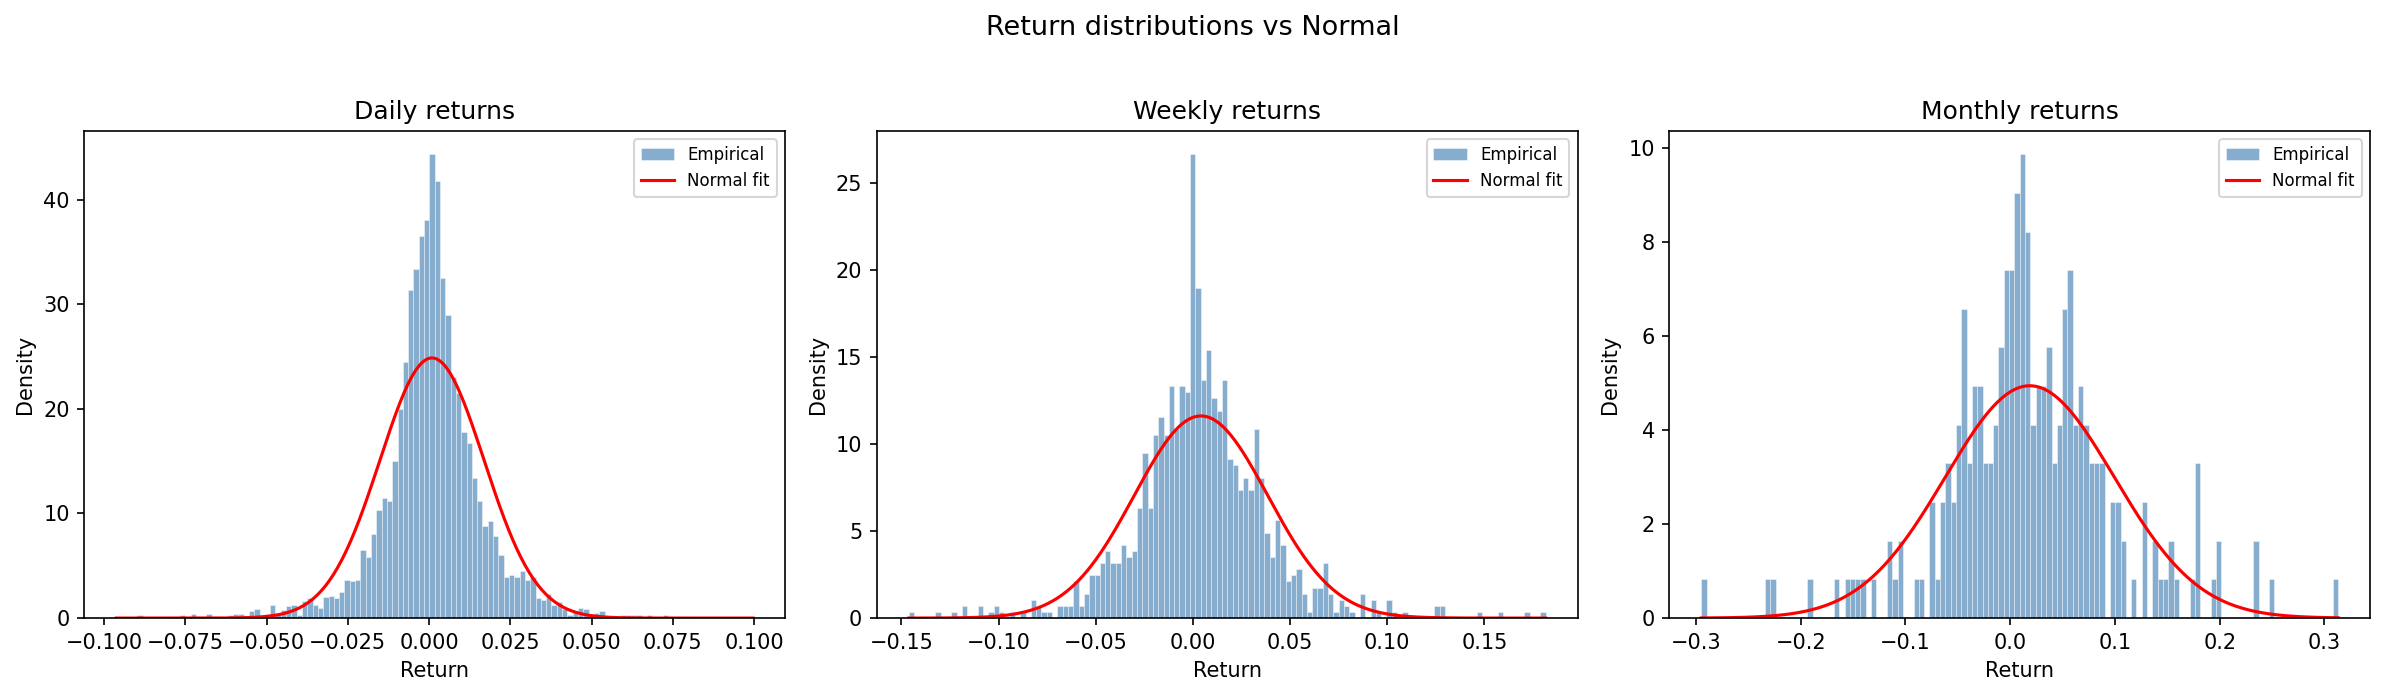
\includegraphics[width=0.9\textwidth]{../main/eda_result/01_return_histograms.png}
    \caption{Return Distribution: The empirical distribution of market returns exhibits significantly higher peaks and "fatter tails" (excess kurtosis) than the normal distribution overlay.}
    \label{fig:ret_hist}
\end{figure}

The Jarque-Bera test confirms this deviation from normality, with significant skewness and kurtosis that indicate a higher probability of extreme "black swan" events than predicted by a Random Walk model. As shown in Table~\ref{tab:summary_stats}, the excess kurtosis across all frequencies significantly exceeds the Gaussian baseline of zero, particularly for daily returns (4.7286). This non-normality is further visualized in the QQ-plot (Figure~\ref{fig:qq_plot}), where the "S-curve" shape at the extremes denotes the presence of heavy tails.

\begin{table}[H]
    \centering
    \small
    \caption{Summary Statistics and Normality Tests for Market Returns (2006--2025)}
    \label{tab:summary_stats}
    \begin{tabular}{lrrrrrrr}
    \toprule
    \textbf{Frequency} & \textbf{N} & \textbf{Mean (\%)} & \textbf{Vol (\%)} & \textbf{Skew} & \textbf{Kurt} & \textbf{JB Stat} & \textbf{p-val} \\
    \midrule
    Daily   & 4859 & 0.0888 & 1.6040 & -0.1856 & 4.7286 & 4543.12 & 0.0000 \\
    Weekly  & 1044 & 0.4123 & 3.4349 & 0.2610  & 3.3328 & 488.73  & 0.0000 \\
    Monthly & 240  & 1.8708 & 8.0710 & 0.0102  & 2.0894 & 40.86   & 0.0000 \\
    \bottomrule
    \end{tabular}
\end{table}

\begin{figure}[H]
    \centering
    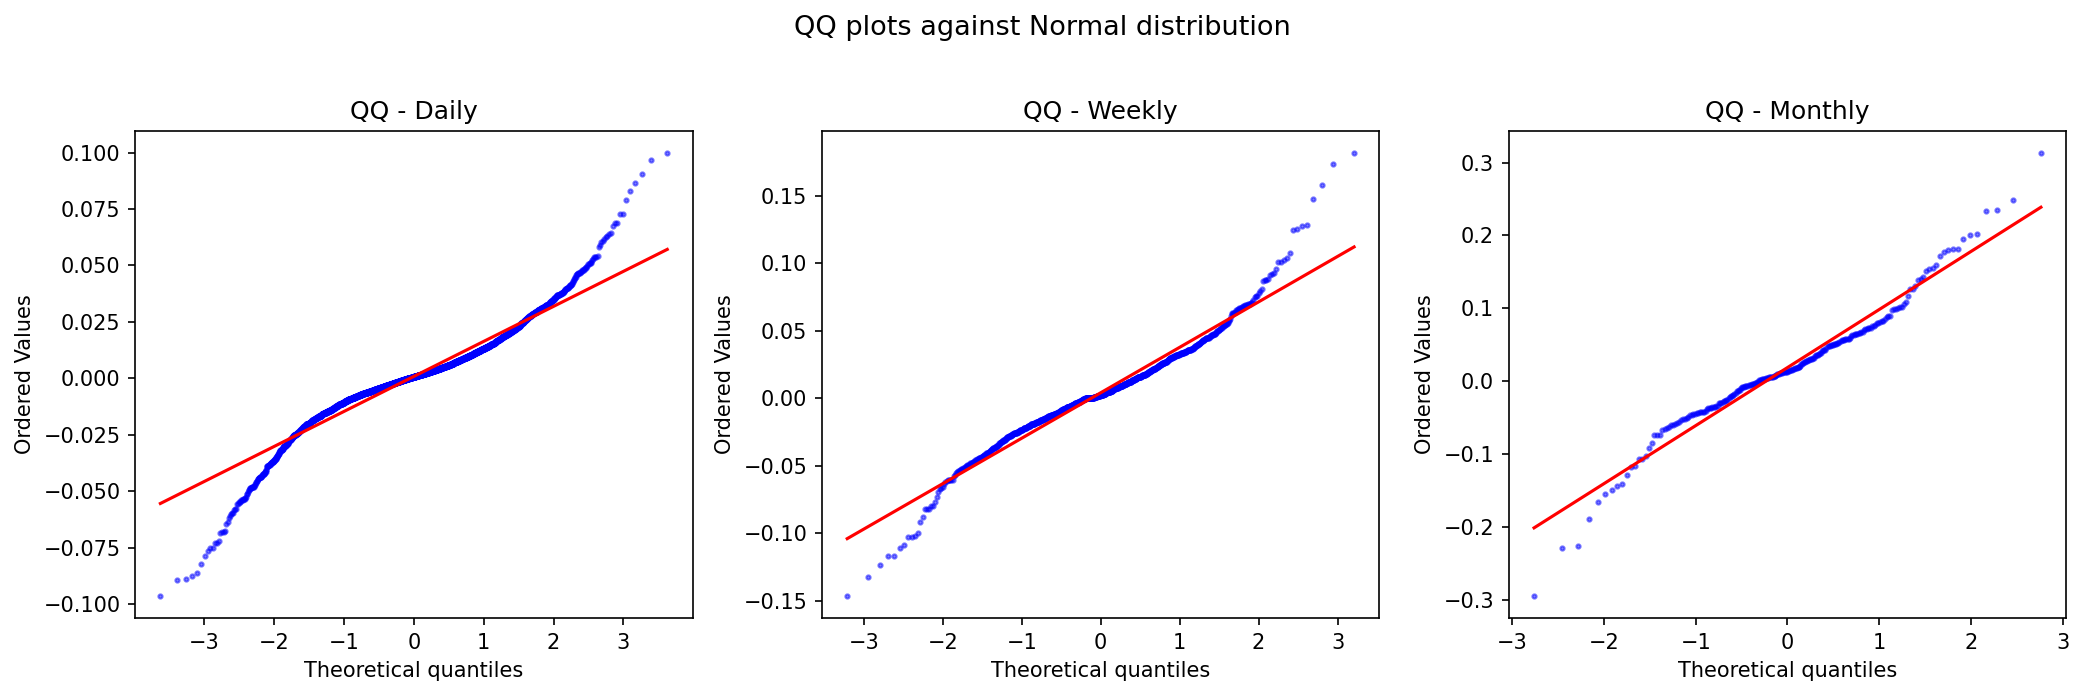
\includegraphics[width=0.75\textwidth]{../main/eda_result/02_qq_plots.png}
    \caption{Quantile-Quantile (QQ) Plot: Significant deviations from the diagonal at the tails confirm that market returns are not Gaussian.}
    \label{fig:qq_plot}
\end{figure}

\subsubsection{Volatility Clustering and Autocorrelation}
A core motivation for the HMM is "volatility clustering"—the tendency for large price changes to be followed by further large price changes. This phenomenon strongly motivates the use of an HMM to capture prolonged periods of high or low volatility, which are unobserved but can be inferred from price action.

\begin{figure}[H]
    \centering
    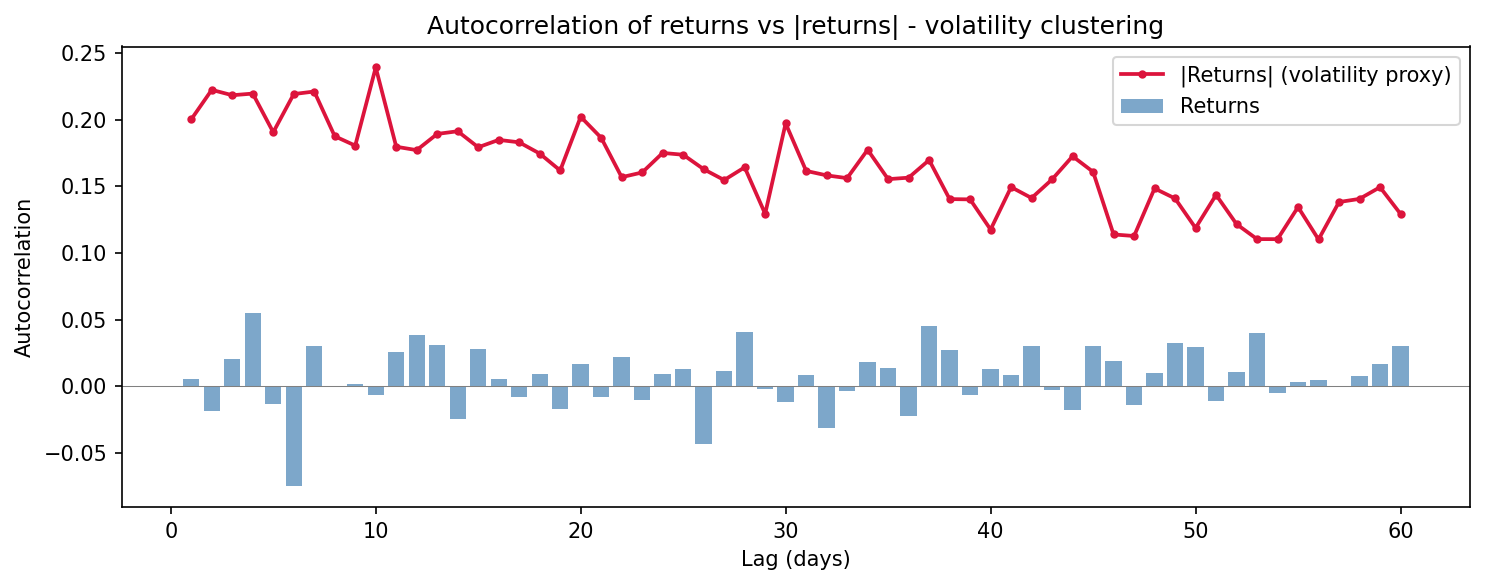
\includegraphics[width=0.9\textwidth]{../main/eda_result/04_autocorrelation.png}
    \caption{Autocorrelation Analysis: While raw returns (left) show little autocorrelation, the squared or absolute returns (right) show strong, persistent autocorrelation. This perfectly visualizes the volatility clustering effect, justifying the transition from a constant-parameter random walk to a regime-switching framework.}
    \label{fig:autocorr}
\end{figure}

\subsubsection{Market Regime Characterization}
The implementation of the Hidden Markov Model (HMM) provides a probabilistic lens through which to view structural shifts in market behavior. This analysis characterizes the transition between low-volatility "Efficient" states and high-volatility "Panic" states.

\begin{figure}[H]
    \centering
    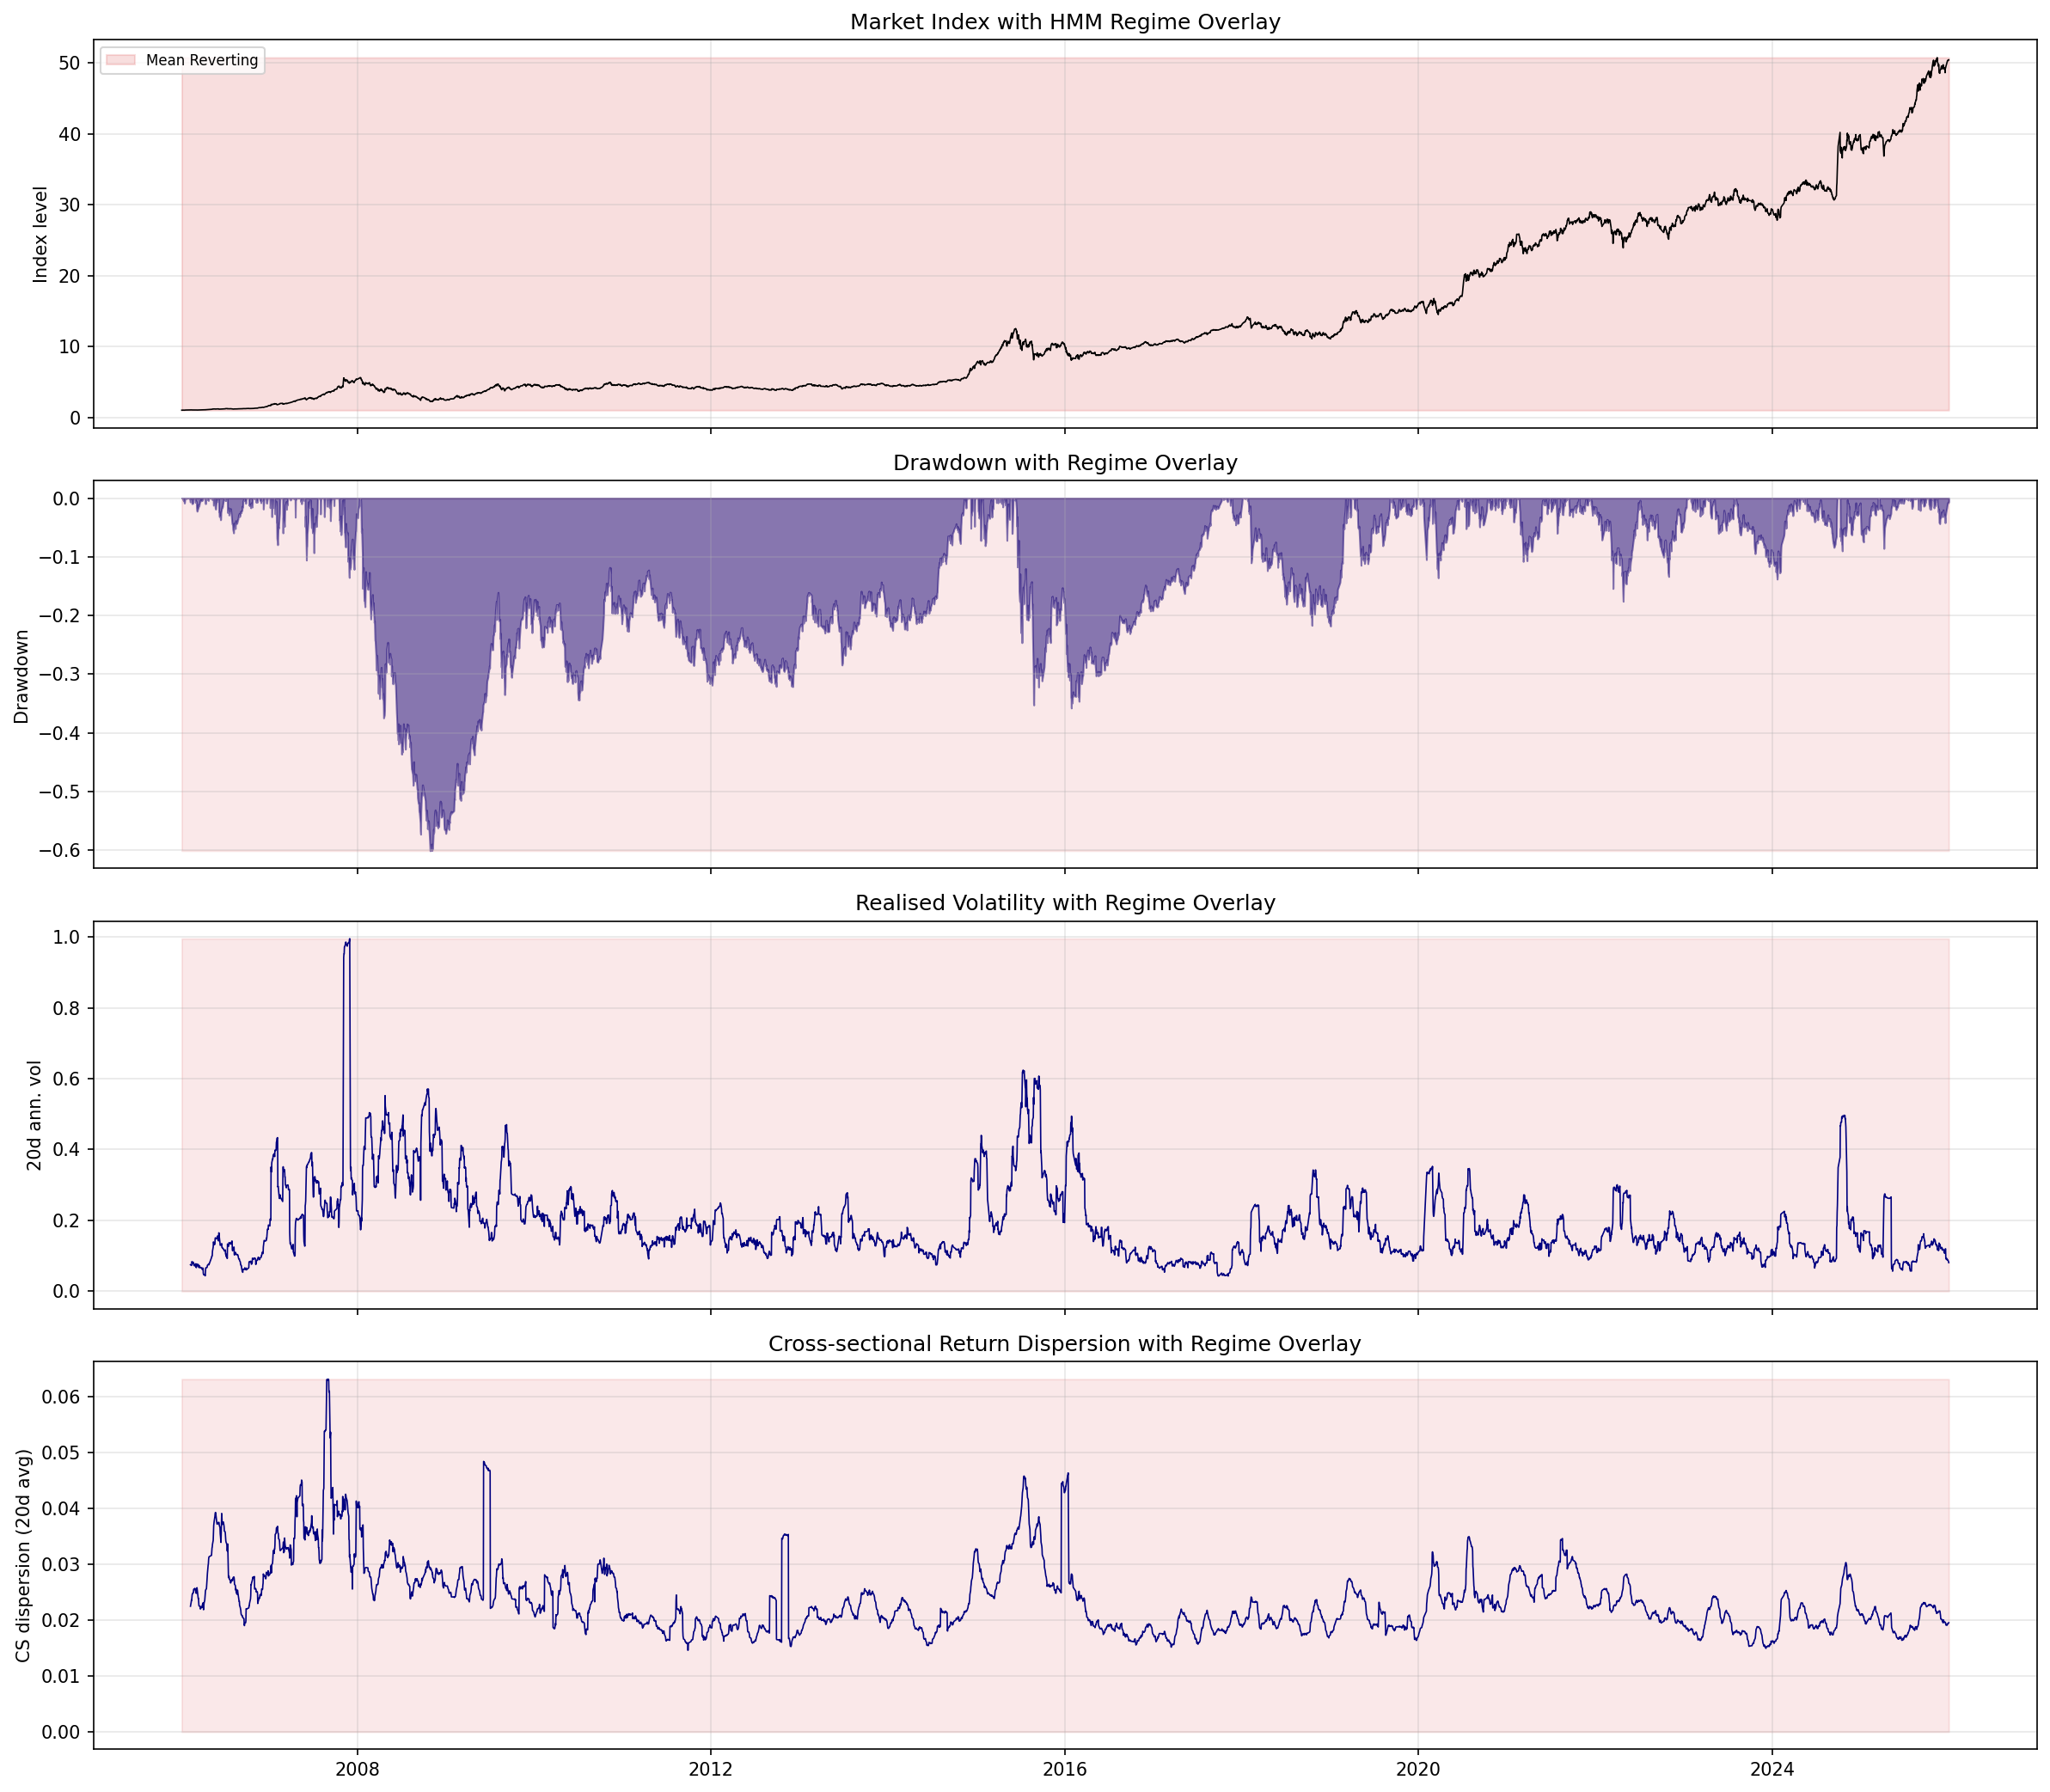
\includegraphics[width=0.95\textwidth]{../main/eda_result/25_regime_context.png}
    \caption{Market Regime Context: This visualization overlays the HMM's state classification on the Market Index, drawdowns, realized volatility, and cross-sectional dispersion. It demonstrates the model's ability to identify regime shifts in real-time, matching the qualitative "feel" of market panics with quantitative state transitions.}
    \label{fig:regime_context}
\end{figure}

The robust classification seen in Figure \ref{fig:regime_context} is further supported by the \textbf{HMM Transition Matrix}. Our empirical results show that market states are significantly "sticky," meaning that once the market enters a specific regime, it has a high mathematical probability of remaining there for a prolonged period.

\begin{figure}[H]
    \centering
    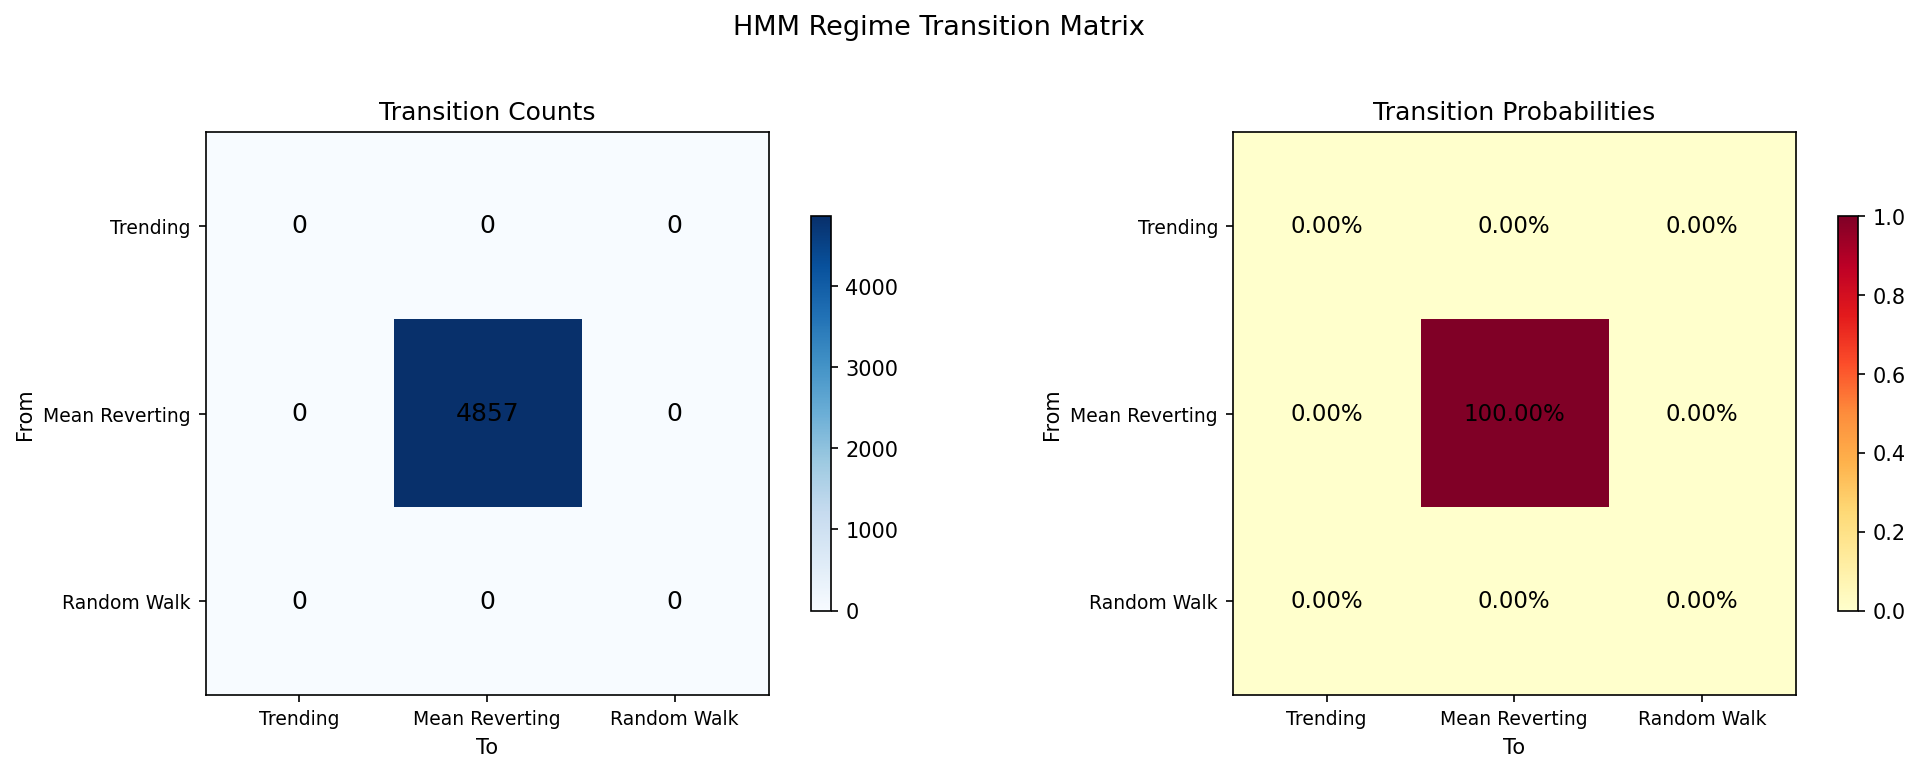
\includegraphics[width=0.75\textwidth]{../main/eda_result/26_transition_matrix.png}
    \caption{HMM Transition Matrix: The high diagonal probabilities confirm that regimes are persistent. This justifies our strategy's medium-term outlook, as the detected state is likely to persist long enough for capital allocation to be effective.}
    \label{fig:transition_matrix}
\end{figure}

The necessity of this adaptive approach is best illustrated by the historical oscillation of volatility. As shown in Figure \ref{fig:mcw_vol}, the market frequently experiences sudden "panic-driven" spikes---most notably during the 2015 deleveraging crisis and the 2020 COVID-19 crash---which traditional linear models fail to accommodate.

\begin{figure}[H]
    \centering
    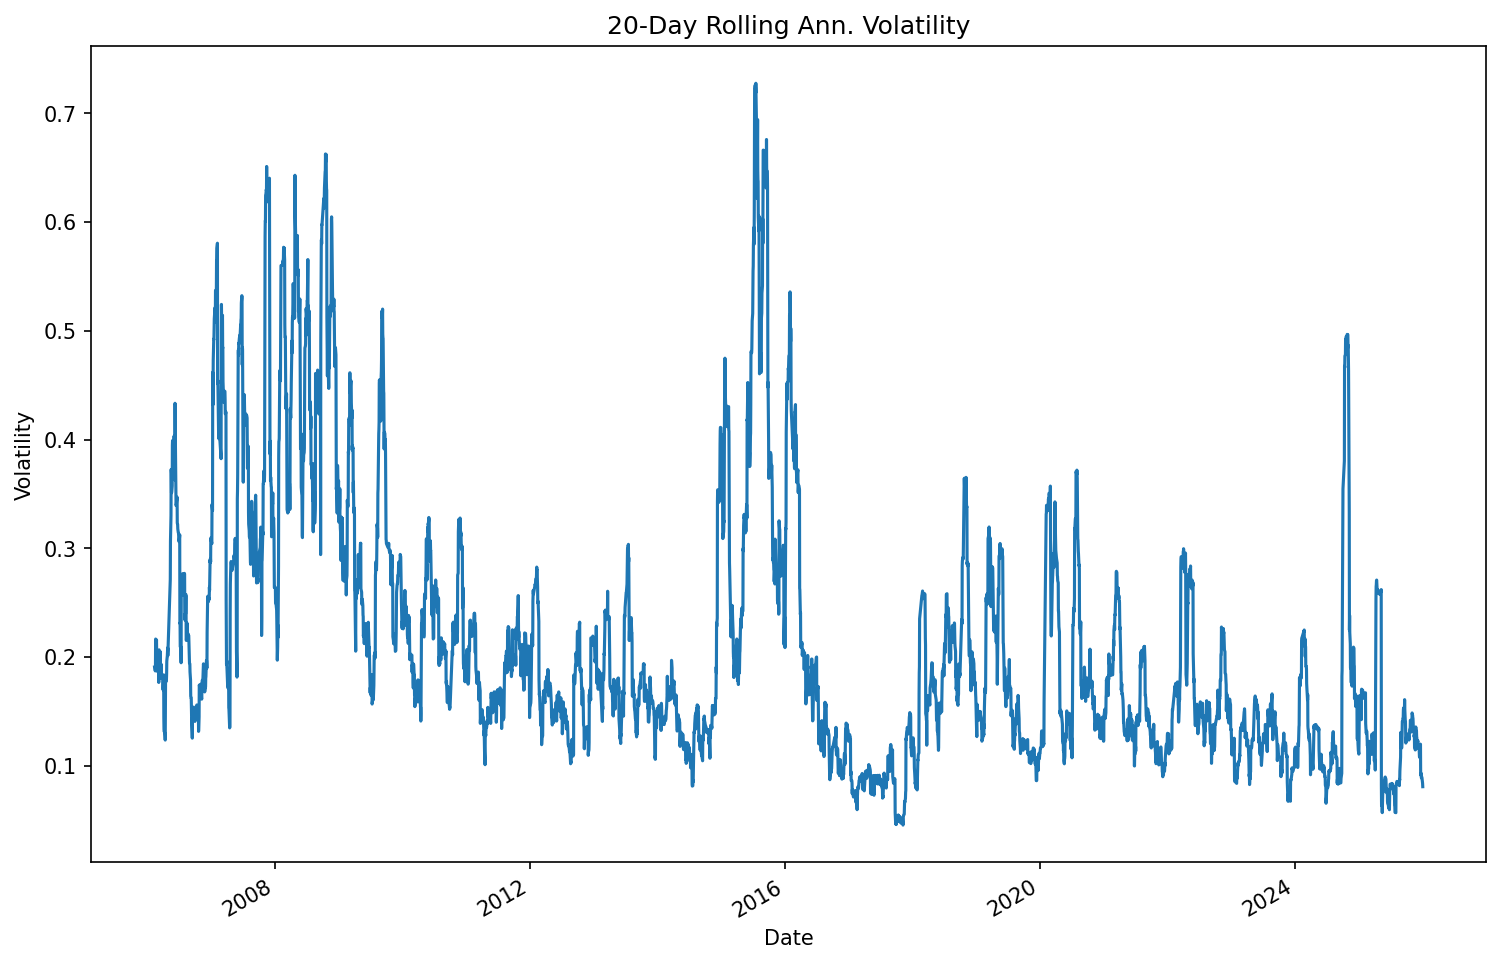
\includegraphics[width=0.9\textwidth]{../main/eda_result/00_mcw_vol.png}
    \caption{Market Cap Weighted (MCW) Volatility: Standardized rolling volatility depicts the drastic shifts between stable growth and extreme market stress, providing the empirical baseline for the HMM's switching logic.}
    \label{fig:mcw_vol}
\end{figure}

Finally, we analyze how strategy factors behave across these detected states. As seen in Figure \ref{fig:factor_regime}, momentum efficacy is heavily dependent on the underlying regime, with the highest alpha generated during persistent "Trending" states ($H > 0.55$).

\begin{figure}[H]
    \centering
    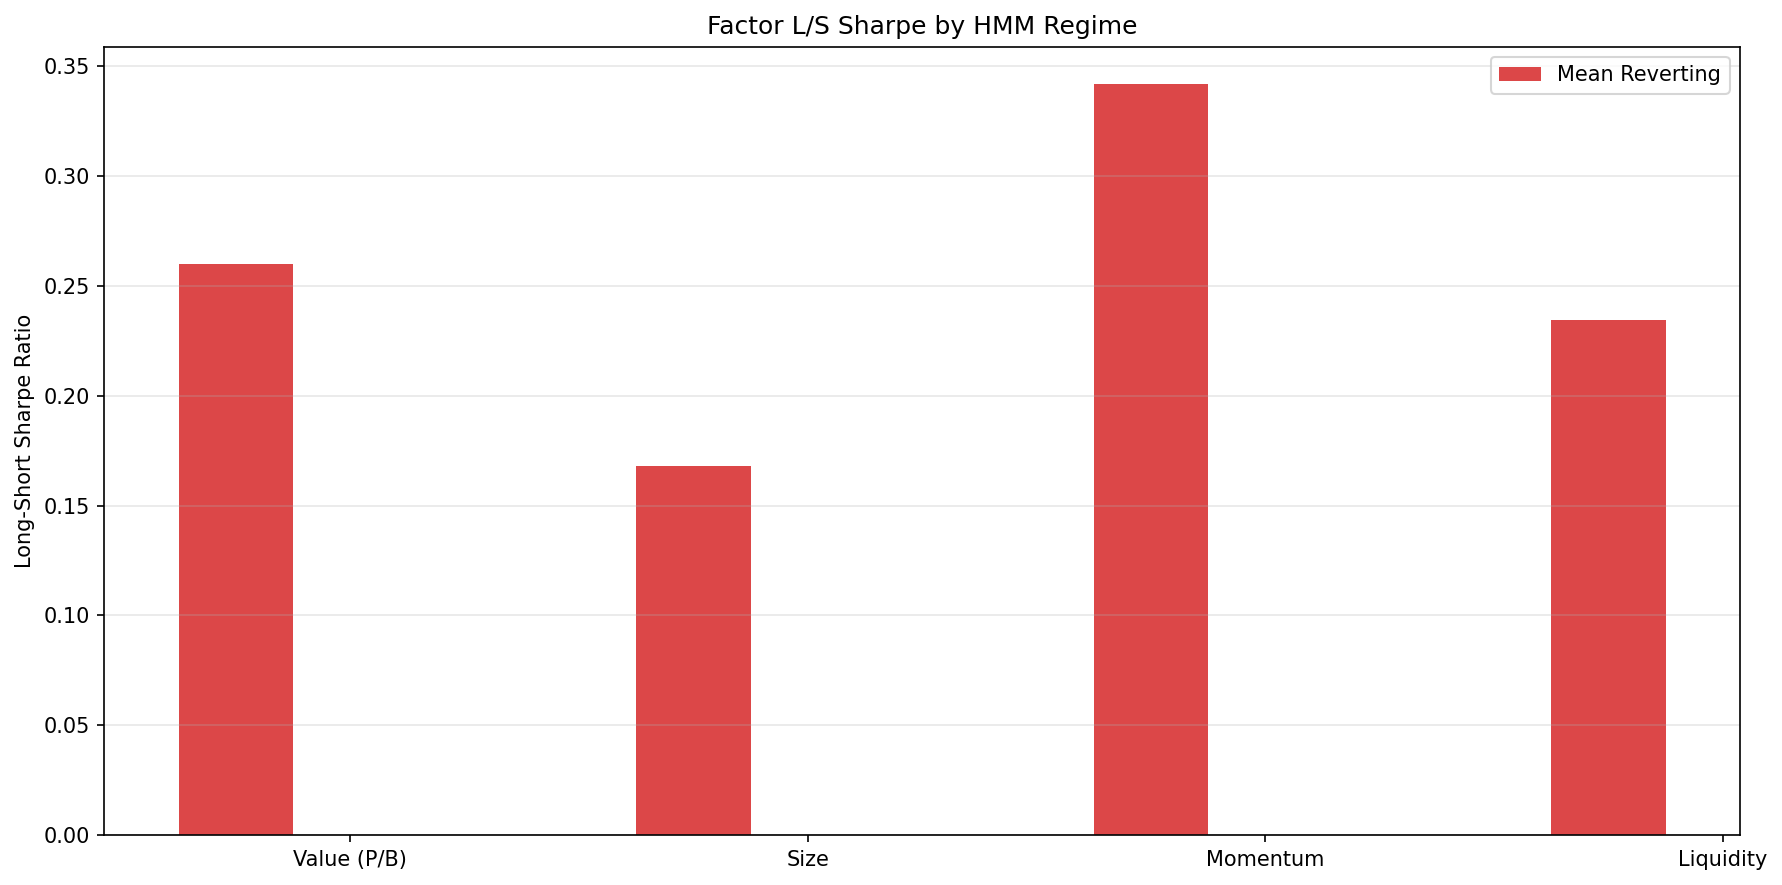
\includegraphics[width=0.8\textwidth]{../main/eda_result/27_factor_by_regime.png}
    \caption{Conditional Factor Performance: Comparison of Strategy Sharpe Ratios across HMM regimes.}
    \label{fig:factor_regime}
\end{figure}

\subsubsection{Baseline Momentum Factor Performance}
Before implementing the HMM-regime filters, it is essential to establish the baseline performance of the momentum factor within our investable universe. 

\begin{figure}[H]
    \centering
    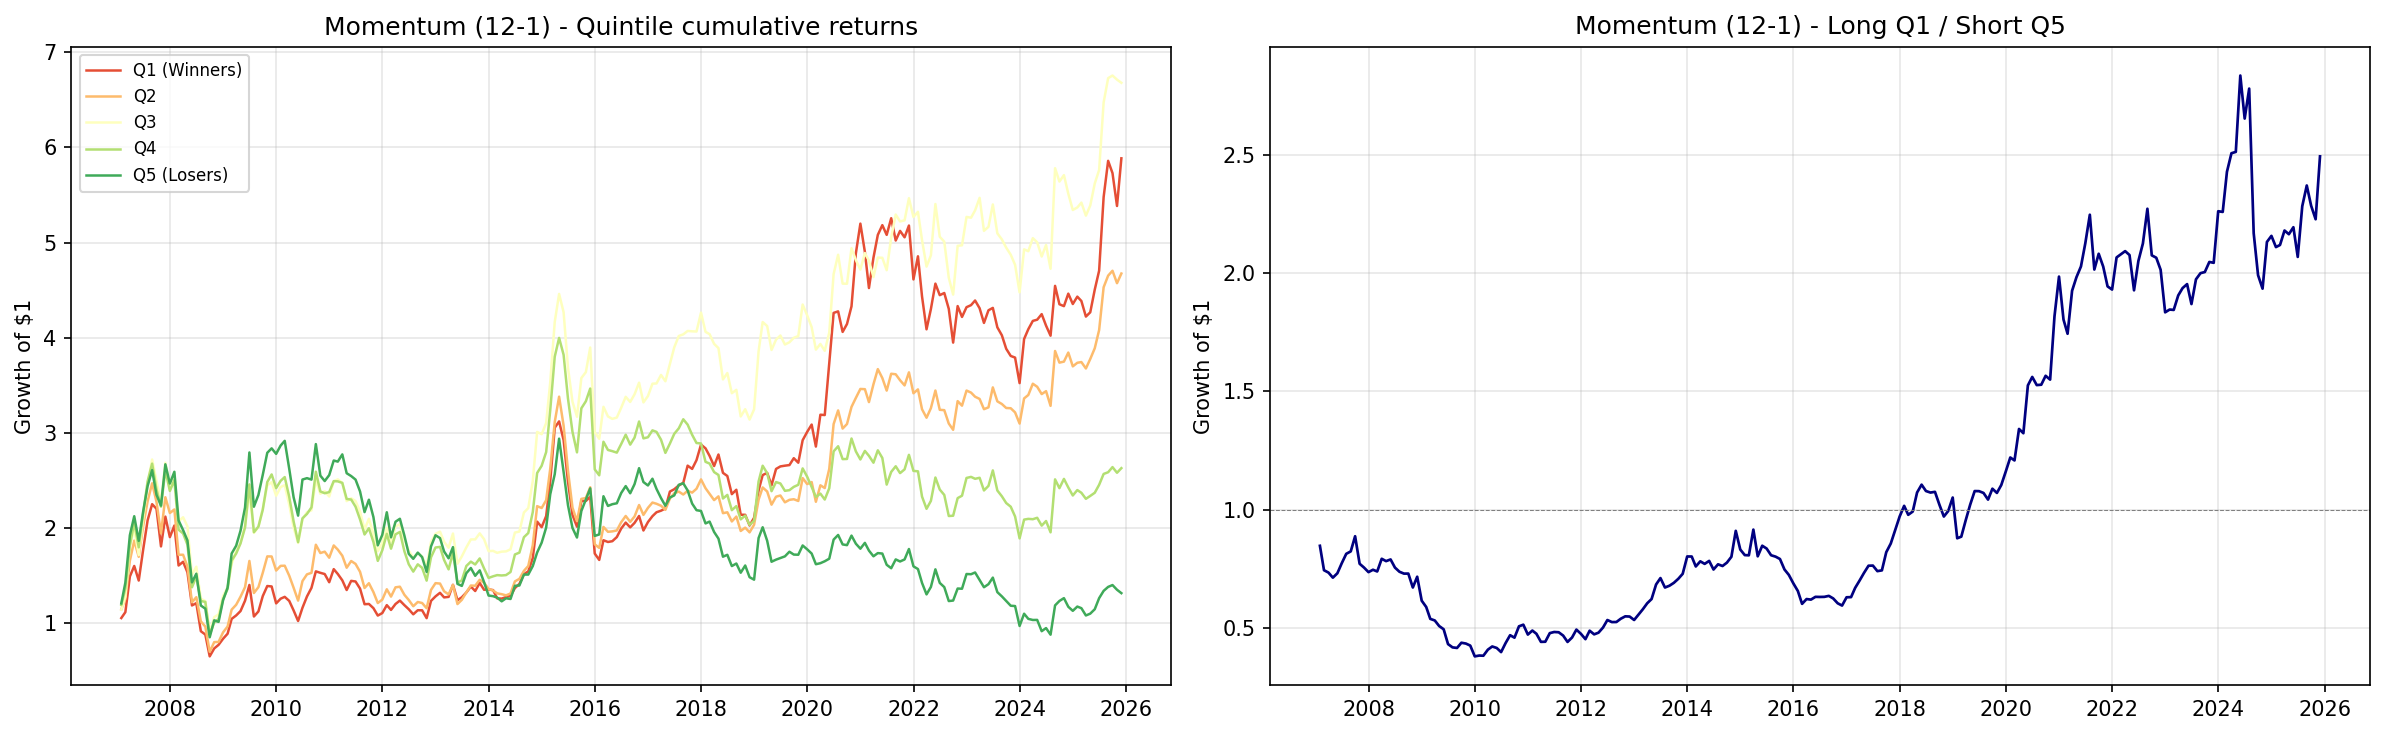
\includegraphics[width=0.9\textwidth]{../main/eda_result/09_factor_momentum.png}
    \caption{Momentum Factor Performance: Cumulative returns of winners (Q1) vs. losers (Q5) and the resulting long/short spread. This establishes the raw alpha available before sophisticated filtering.}
    \label{fig:mom_benchmark}
\end{figure}

The analysis in Figure \ref{fig:mom_benchmark} reveals that while momentum exhibits periods of significant outperformance, it is subject to sharp "reversals" and prolonged underperformance during market dislocations. As shown previously in Figure \ref{fig:factor_regime}, the efficacy of this factor---measured by its Long-Short Sharpe ratio---is highly regime-dependent. Specifically, momentum thrives in persistent trending environments but degrades into a random walk or mean-reverting behavior during high-volatility regimes. This empirical evidence provides the final justification for our tripartite framework: using HMM to filter regimes, Hurst to confirm persistence, and Momentum for tactical entry.

\subsubsection{Survivorship Bias and Universe Dynamics}
A common pitfall in quantitative backtesting is survivorship bias, where the exclusion of delisted or failed companies artificially inflates strategy returns. To ensure the robustness of this study, we explicitly track the entry and exit of tickers within our universe.

\begin{figure}[H]
    \centering
    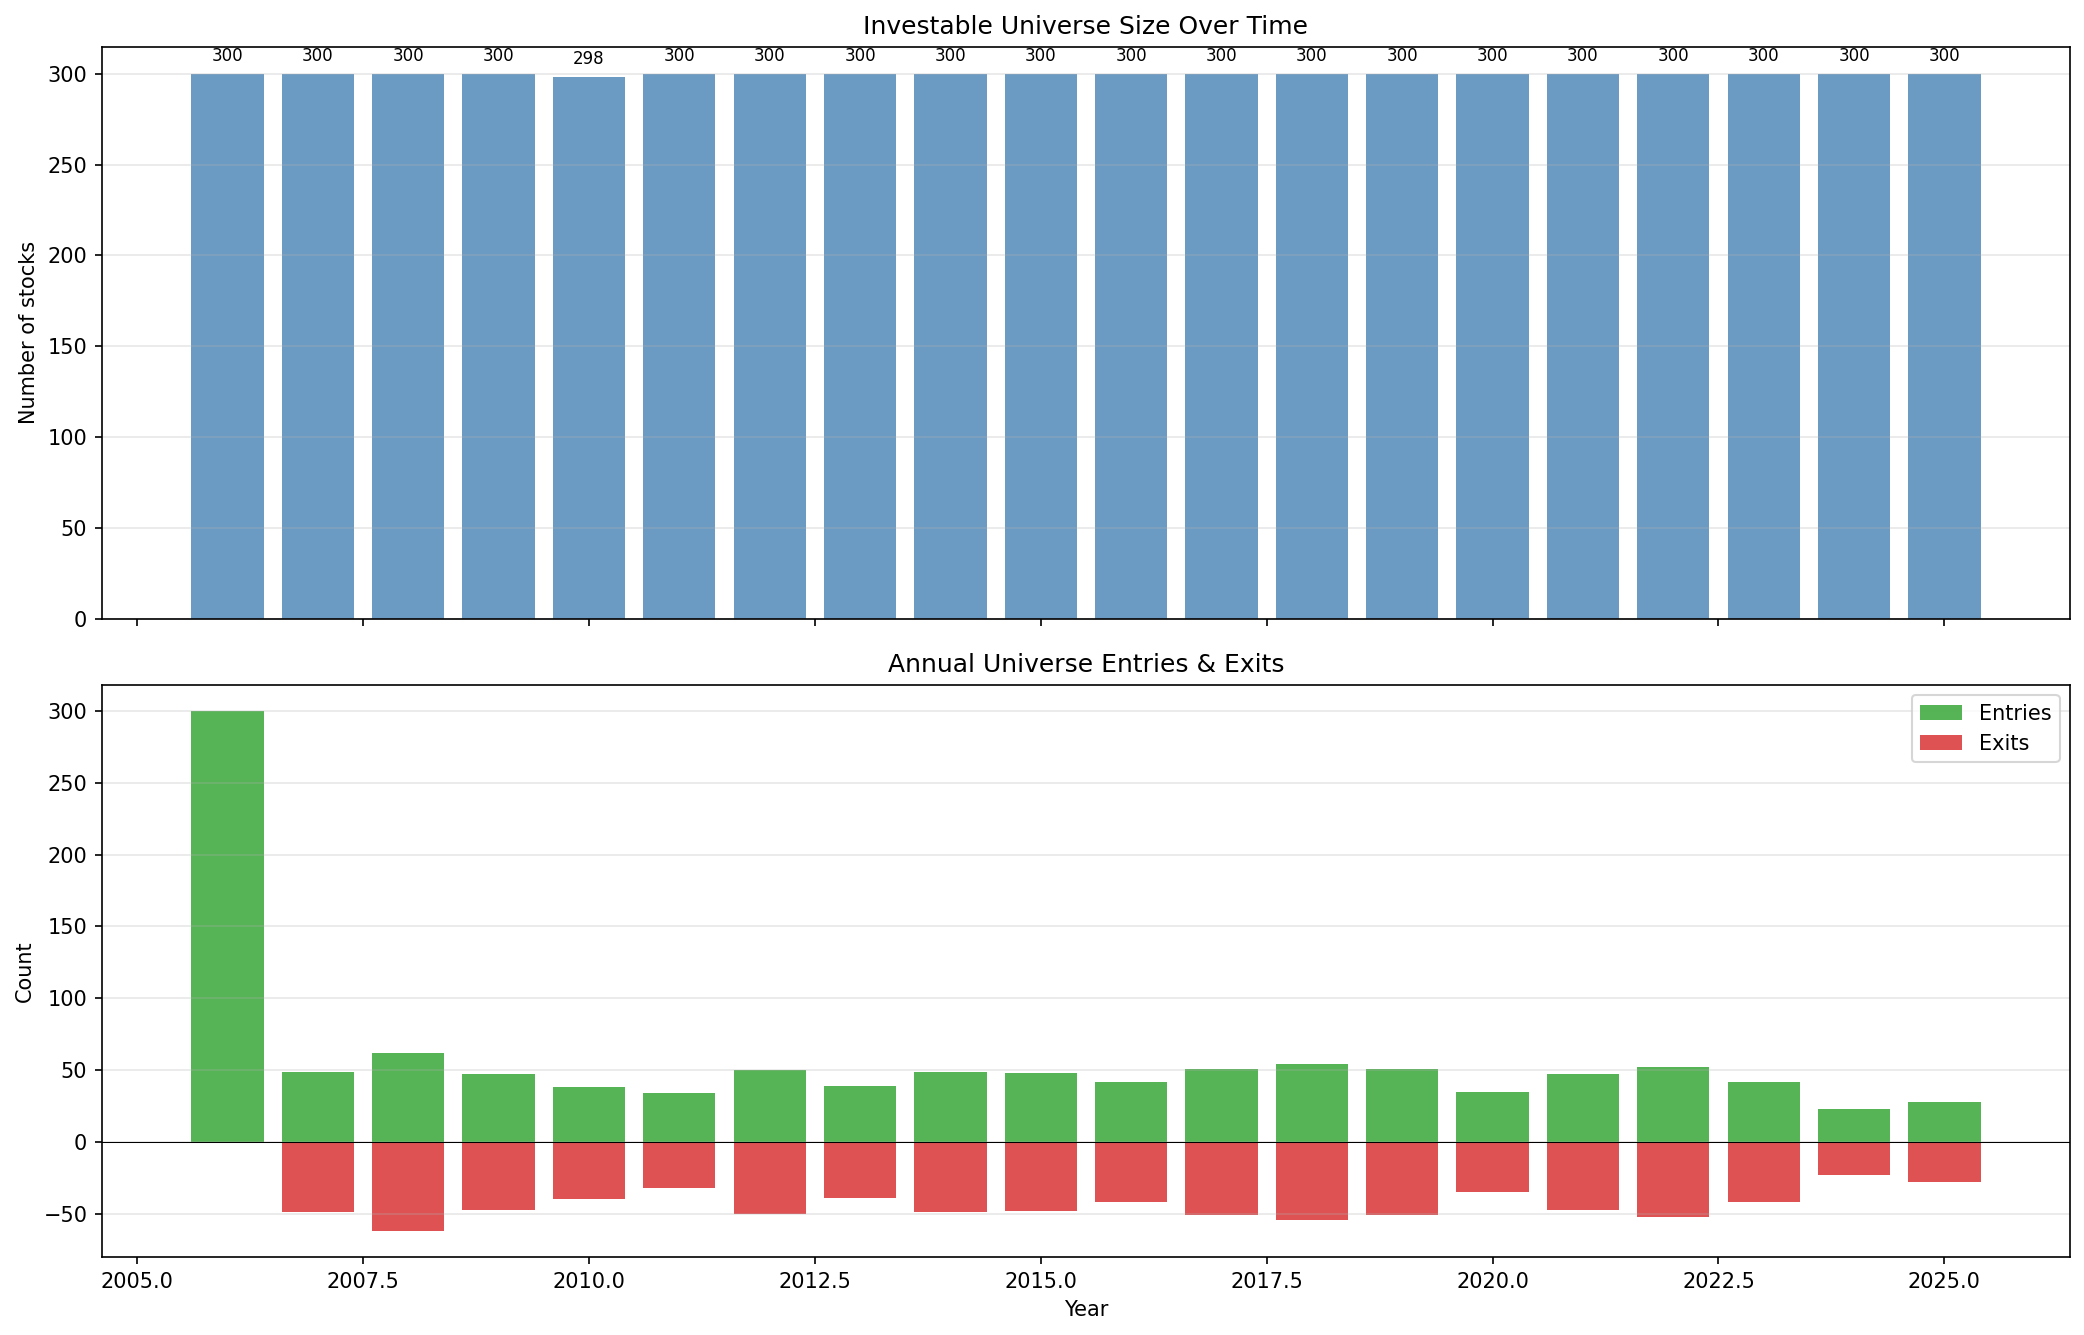
\includegraphics[width=0.9\textwidth]{../main/eda_result/28_universe_dynamics.png}
    \caption{Universe Dynamics: The evolution of the investable universe size alongside annual entries (new listings) and exits (delistings). This confirms that our methodology accounts for the time-varying nature of the market pool.}
    \label{fig:univ_dynamics}
\end{figure}

To quantify the impact of survivorship, we compared the performance of our full investable universe against a "Survivors Only" subset (stocks that existed throughout the entire period). 

\begin{table}[H]
    \centering
    \small
    \caption{Survivorship Bias Impact (2006--2025)}
    \label{tab:survivorship}
    \begin{tabular}{lcccc}
    \toprule
    \textbf{Portfolio Type} & \textbf{Ann. Ret} & \textbf{Ann. Vol} & \textbf{Sharpe} & \textbf{Growth} \\
    \midrule
    Full Universe (EW)      & 0.144 & 0.266 & 0.539 & 8.0x \\
    Survivors Only (EW)     & 0.210 & 0.249 & 0.842 & 31.2x \\
    \midrule
    Full Universe (MCW)     & 0.196 & 0.235 & 0.835 & 25.8x \\
    Survivors Only (MCW)    & 0.224 & 0.255 & 0.879 & 39.9x \\
    \bottomrule
    \end{tabular}
\end{table}

As shown in Table \ref{tab:survivorship} and Figure \ref{fig:surv_bias}, ignoring delistings would nearly triple the cumulative growth in an equal-weight portfolio. By utilizing a point-in-time constituent matrix, our backtesting framework avoids this inflation and reflects a realistic investable opportunity set.

\begin{figure}[H]
    \centering
    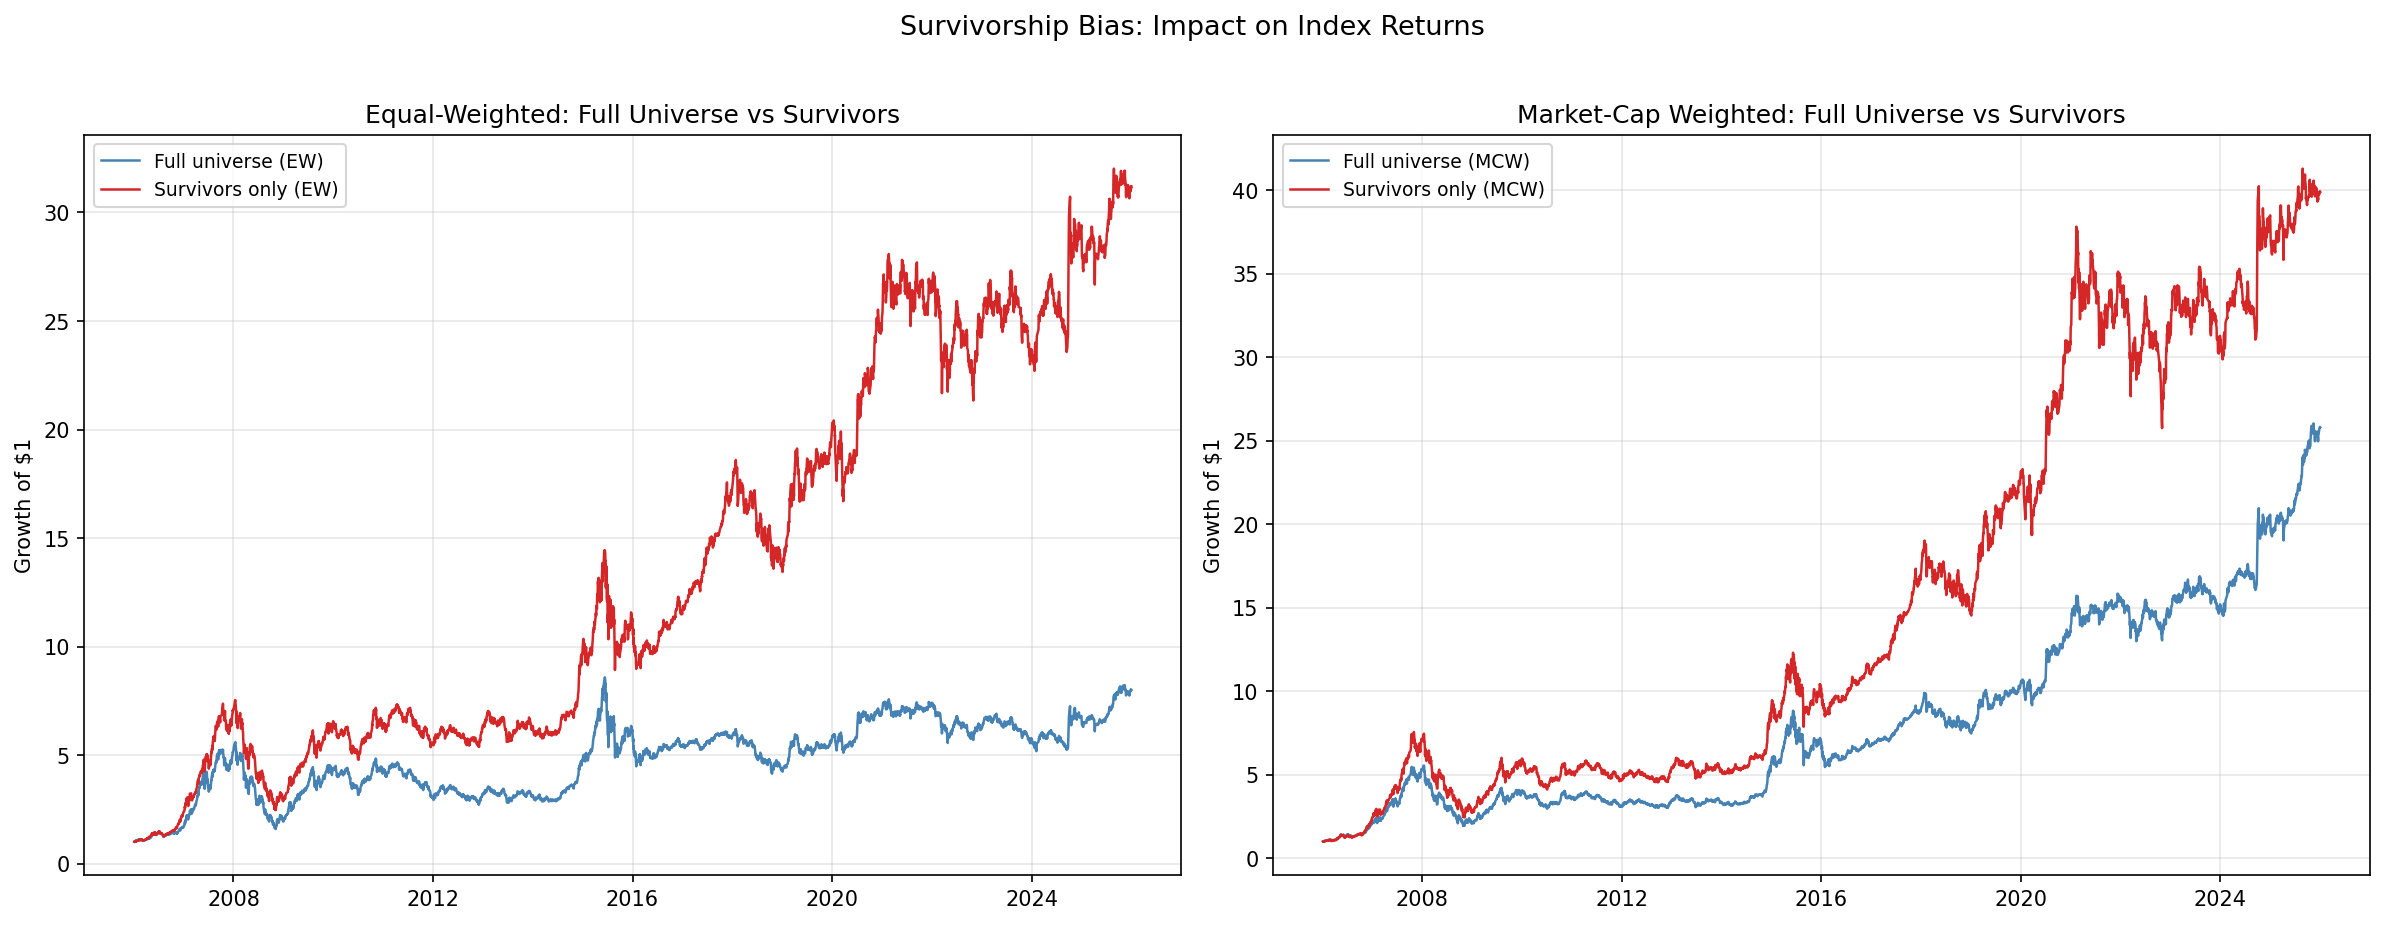
\includegraphics[width=0.85\textwidth]{../main/eda_result/30_survivorship_bias.png}
    \caption{Survivorship Bias Visualization: Performance gap between bias-free and biased universes.}
    \label{fig:surv_bias}
\end{figure}

\subsubsection{Liquidity and Market Microstructure}
The practical implementation of a quantitative strategy is constrained by market liquidity. Our HMM's decision to shift into cash during high-volatility regimes is further justified by the breakdown of liquidity during market stress events.

\begin{figure}[H]
    \centering
    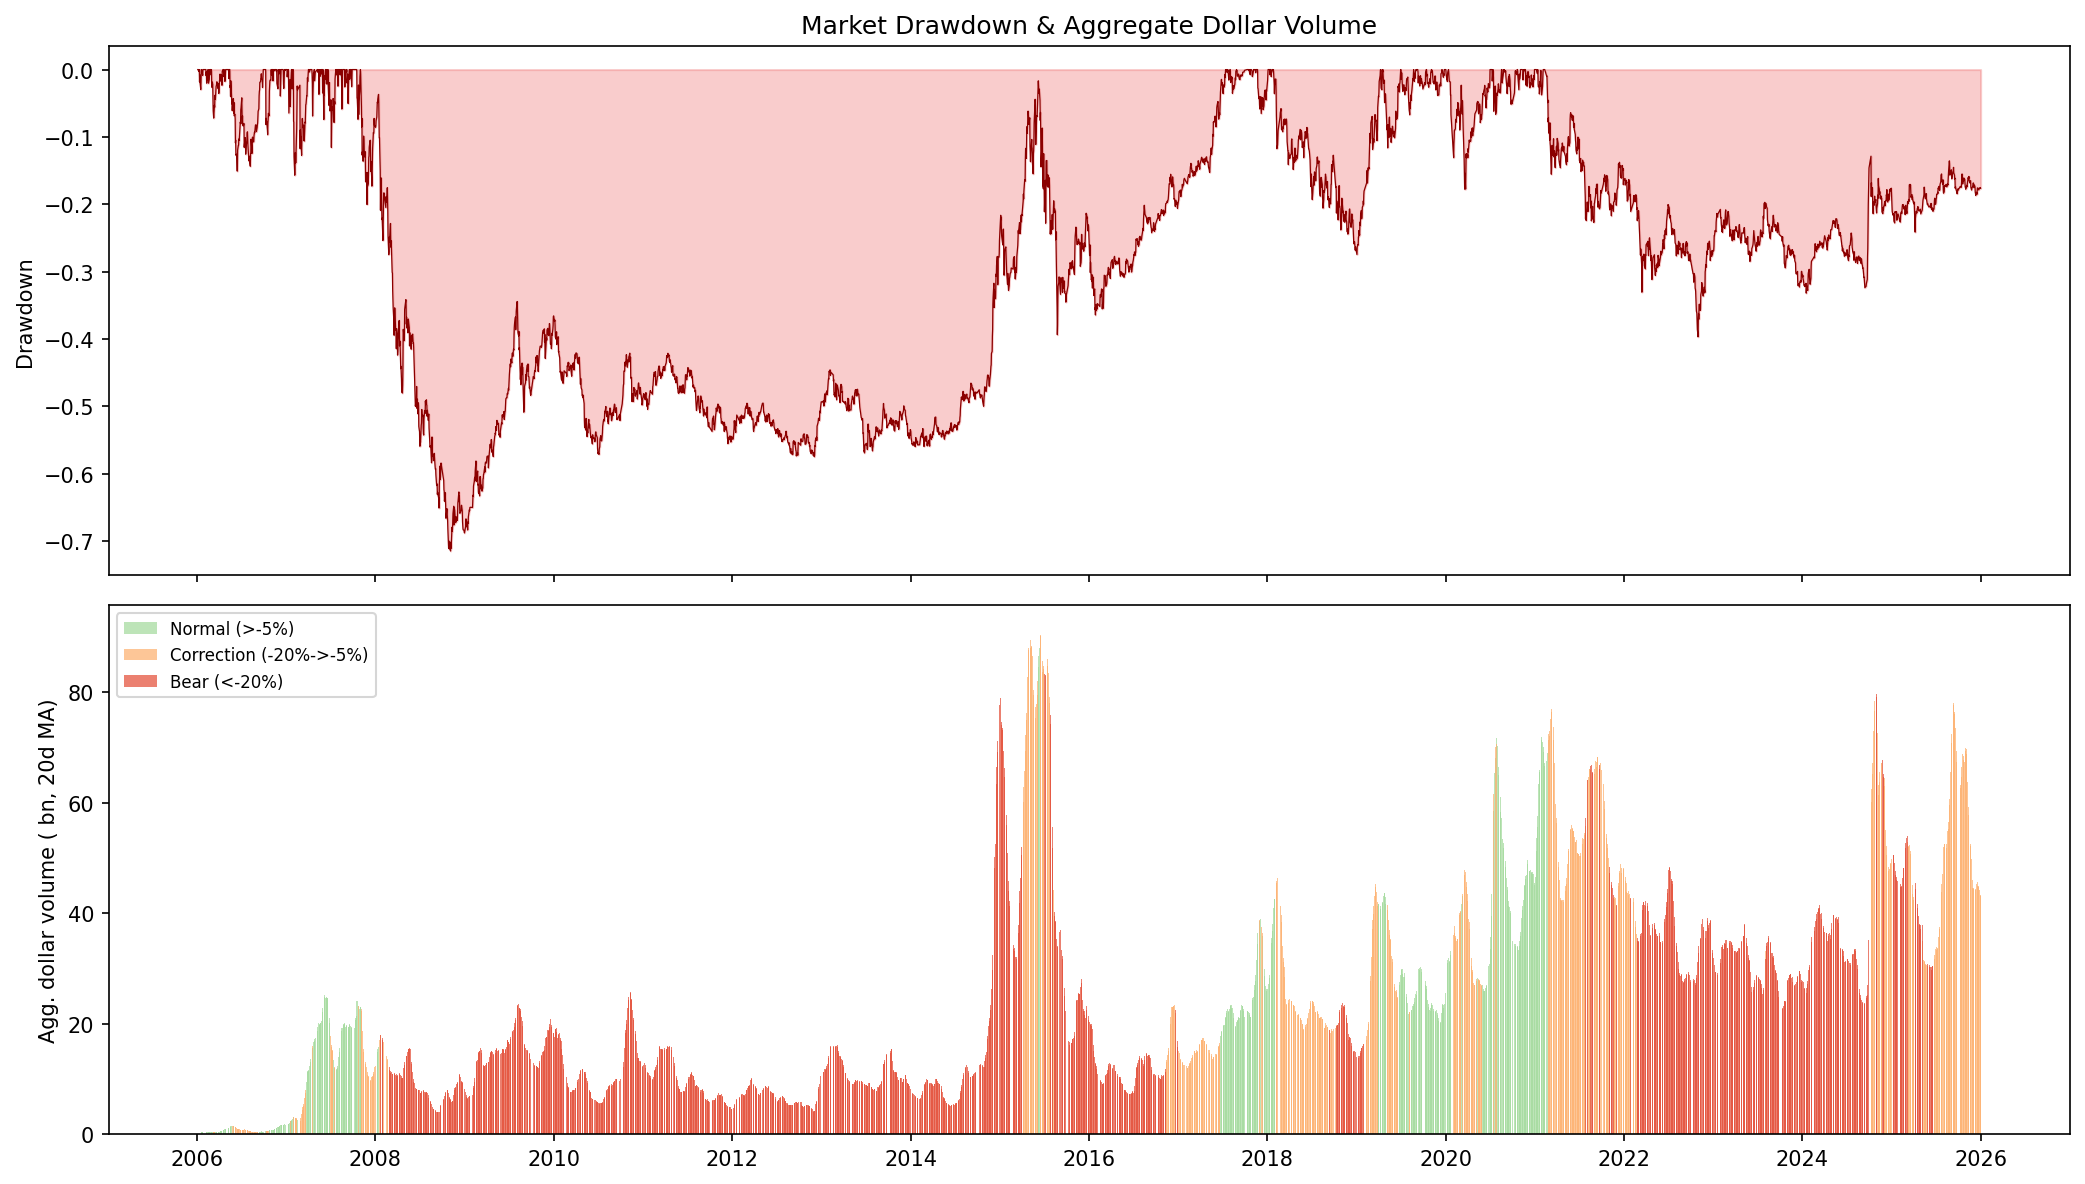
\includegraphics[width=0.9\textwidth]{../main/eda_result/19_liquidity_drawdowns.png}
    \caption{Liquidity vs. Drawdowns: The relationship between aggregate market dollar volume and price drawdowns. Note how liquidity significantly contracts during the deepest phases of market crashes.}
    \label{fig:liq_drawdown}
\end{figure}

Using the Amihud illiquidity ratio (Figure \ref{fig:amihud}), we observe that execution costs and slippage risk skyrocket during the high-volatility states identified by the HMM. This provides a fundamental microstructural rationale for our "Safe Harbor" rule: during periods of extreme illiquidity and high volatility, the safest tactical move is to reduce exposure to avoid the high costs of "distressed" trading.

\begin{figure}[H]
    \centering
    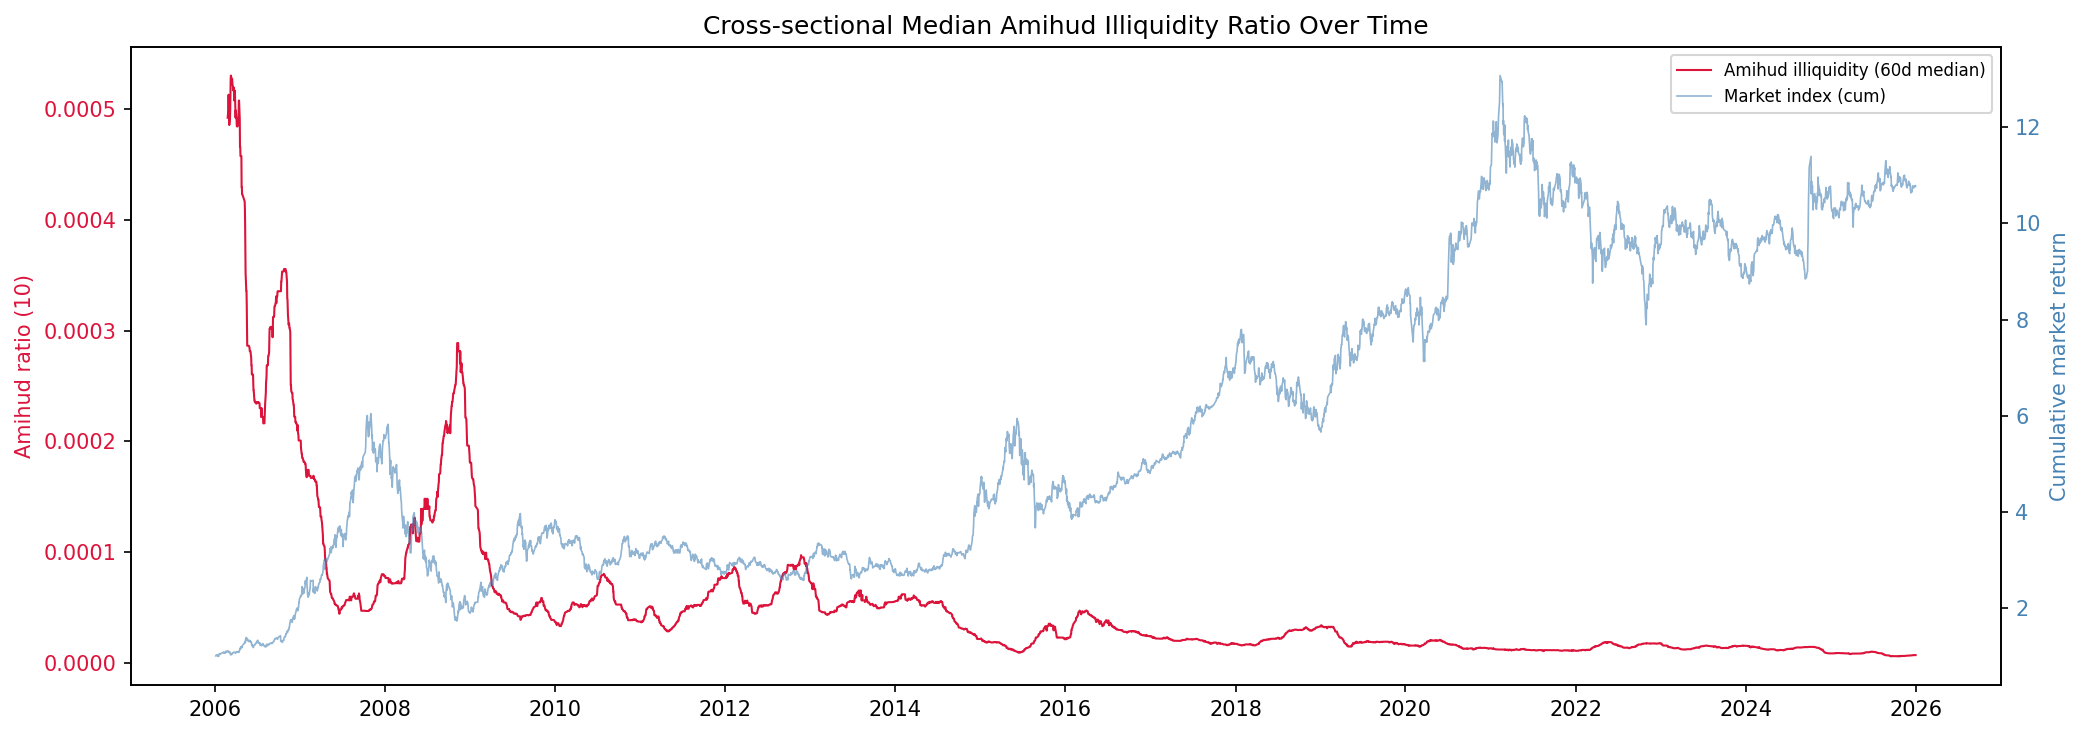
\includegraphics[width=0.85\textwidth]{../main/eda_result/17_amihud_illiquidity.png}
    \caption{Amihud Illiquidity Ratio: Cross-sectional median ratio over time. Spikes in illiquidity perfectly align with the HMM's high-volatility state transitions.}
    \label{fig:amihud}
\end{figure}

\subsubsection{Hurst Exponent}

The Figure~\ref{fig:hurst_000031} presents the adjusted closing prices, sector-neutral log returns, and rolling Hurst exponent for a sample Chinese equity. The price exhibits an upward trend between 2014 and 2016, and it was followed by a prolonged decline and stabilization. This period coincides with elevated Hurst exponent values above 0.6, which implies strong persistence and trending behavior. On the other hand, the post-2020 period is characterized by Hurst values predominantly below 0.5, which implies the mean-reverting dynamics. The log return series reveals volatility clustering, especially during trending phase. Overall, the evidence supports the presence of time-varying market regimes, therefore it highlights the importance of adaptive training strategies.

\begin{figure}[H]
    \centering
    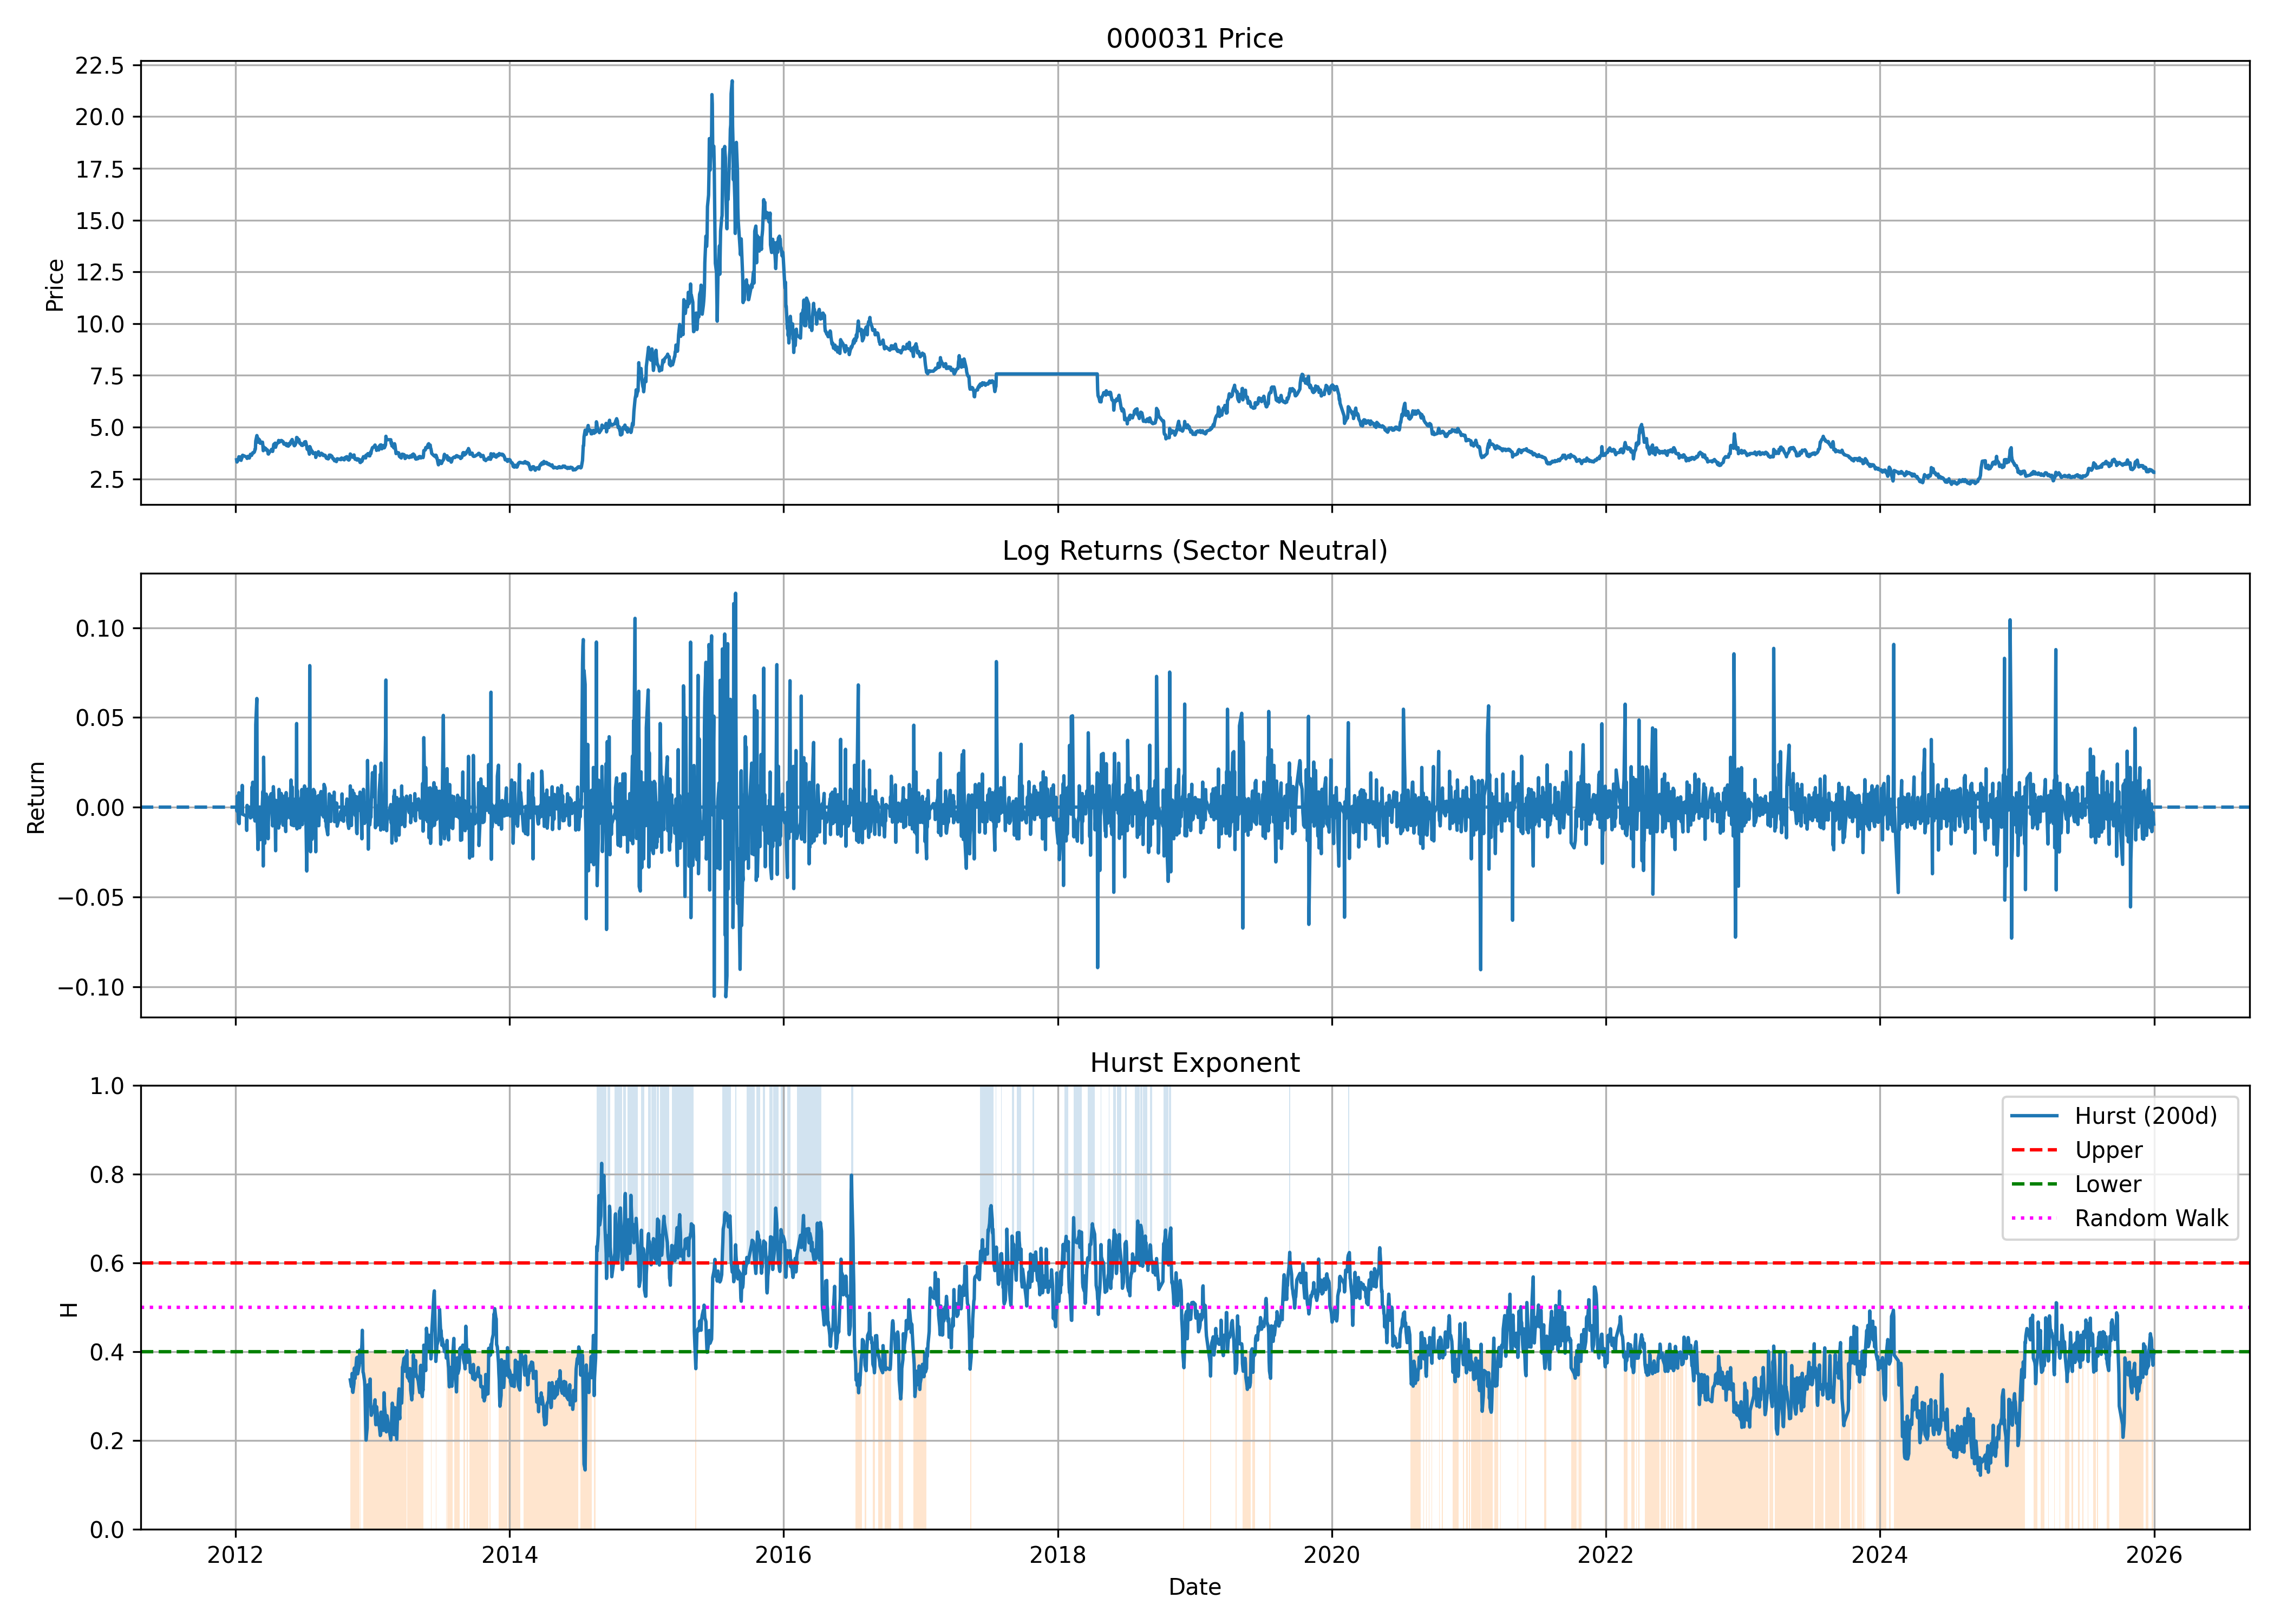
\includegraphics[width=0.85\textwidth]{../main/backtest_result/hurst_full_000031.png}
    \caption{Price, Log Return and Hurst Exponent of a sample stock}
    \label{fig:hurst_000031}
\end{figure}


\subsection{Backtesting Framework}

To rigorously evaluate the empirical viability of the HMM-Hurst-Momentum strategy, we developed an event-driven historical simulation engine. Unlike standard vectorized backtests, which often implicitly assume frictionless execution and fractional shares, our framework strictly enforces temporal causality and market microstructural constraints to prevent look-ahead bias and accurately reflect live trading conditions.

\subsubsection{Portfolio Weighting Schemas}
The translation of a discrete trading signal $S_{i,t} \in \{-1, 0, 1\}$ into an actionable target portfolio weight $w_{i,t}$ is a critical determinant of strategy performance. The framework supports multiple weighting schemas:

\begin{enumerate}
    \item \textbf{Market-Capitalization Weighting (Standard):} Capital is allocated proportionally to the lagged market capitalization of the assets generating active signals. A survivorship-bias-free constituent mask is applied daily to ensure only assets within the tradable universe at time $t$ are considered.
    
    \item \textbf{Inverse Volatility (VaR Parity):} To achieve a constant risk budget, target weights are determined inversely to their forecasted downside risk. Using the 1-day 99\% EWMA Value-at-Risk ($\text{VaR}_{i,t}$), the weight is defined as:
    $$ w_{i,t} = S_{i,t} \left( \frac{\text{Target Risk}}{\text{VaR}_{i,t-1}} \right) $$
    where the Target Risk budget is capped to prevent portfolio leverage from exceeding 1.0.
\end{enumerate}

\subsubsection{Microstructural Constraints and Frictions}
To ensure the backtest reflects the realities of the Chinese A-share market, specific execution frictions and constraints were hard-coded into the trading simulator:

\begin{itemize}
    \item \textbf{Transaction Costs and Stamp Duty:} We impose an asymmetric cost structure mirroring standard Chinese brokerage accounts. Executed buy orders incur a 0.03\% fee (comprising broker commission and transfer fees). Sell orders incur a higher 0.08\% fee, accounting for the mandated 0.05\% regulatory stamp duty alongside standard commissions.
    \item \textbf{Board Lot Discretization:} The engine restricts order sizing to integer multiples of standard ``board lots'' (100 shares). Fractional share execution is explicitly prohibited:
    $$ \text{Shares}_{i,t} = 100 \times \left\lfloor \frac{w_{i,t} \times \text{Portfolio Value}_{t}}{100 \times P_{i,t}} \right\rfloor $$
    \item \textbf{Turnover Suppression (Drift Tolerance):} To mitigate the erosion of alpha through micro-transaction spam, the engine enforces a 5\% drift tolerance. Rebalancing trades are only triggered if the target position size deviates from the current holdings by more than 5\%.
\end{itemize}

\subsubsection{Tactical Risk Management (Elder Rules)}
To test the impact of strict capital preservation heuristics, an optional risk-gating module based on Dr. Alexander Elder’s trading frameworks was integrated into the execution logic:
\begin{enumerate}
    \item \textbf{The 2\% Rule:} The maximum gross exposure permitted for any single equity is strictly capped at 2\% of total portfolio equity, forcing diversification regardless of signal strength.
    \item \textbf{The 6\% Rule (Monthly Circuit Breaker):} The portfolio's high-water mark is sampled at the start of each calendar month. If the aggregate equity suffers a drawdown exceeding 6\% within that month, a trading halt is triggered, and no new positions are initiated until the subsequent month.
\end{enumerate}

By combining an event-driven architecture with rigorous localized constraints, this framework provides a highly conservative baseline for the strategy's theoretical Compound Annual Growth Rate (CAGR) and Sharpe Ratio.

\section{Results}
To evaluate the practical viability of the proposed regime-switching architecture, we simulated the execution of the 3-state Hidden Markov Model combined with a 200-day Hurst window and 21-day momentum signal ($H=200, N=3, M=21$). The initial portfolio was seeded with \$100,000,000, and transaction costs were strictly modeled to reflect Chinese A-share commission structures. 

Because naive signal generation often ignores the realities of capital concentration and volatility drag, we tested three distinct execution variants of the HMM-Hurst strategy against a Market-Cap Weighted Benchmark:
\begin{enumerate}
    \item \textbf{Standard HMM:} Capital is allocated dynamically based on market-cap weights but restricted only to assets generating active "Long" or "Short" signals.
    \item \textbf{HMM + Elder Rules:} The standard strategy augmented with strict risk-gating. No single asset exceeds a 2\% portfolio allocation, and trading is halted for a month if the portfolio breaches a 6\% monthly drawdown limit.
    \item \textbf{HMM + VaR Parity:} Capital is allocated using an inverse Value-at-Risk (Risk Parity) framework. Position sizes are dynamically scaled inversely to their 1-day 99\% EWMA GARCH volatility forecast, targeting a constant risk budget.
\end{enumerate}

The backtest was conducted using data between 2020 and 2025, and the execution metrics are summarized in Table~\ref{tab:execution_results}.

\begin{table}[h!]
\centering
\small
\begin{tabularx}{\textwidth}{|X|r|c|c|c|c|}
\hline
\textbf{Execution Strategy} & \textbf{Final Value (\$)} & \textbf{Trades} & \textbf{Win Rate} & \textbf{Max DD} & \textbf{Sharpe} \\
\hline
Buy \& Hold Benchmark & 104,254,479 & 189 & 15.3\% & -33.08\% & -0.03 \\
\hline
Standard HMM & 106,734,053 & 3,576 & 51.0\% & -63.99\% & -0.14 \\
\hline
HMM + Elder Rules & 110,487,111 & 3,574 & 51.5\% & -18.72\% & -0.01 \\
\hline
HMM + VaR Parity & \textbf{140,811,506} & 3,590 & \textbf{51.6\%} & \textbf{-25.32\%} & \textbf{0.59} \\
\hline
\end{tabularx}
\caption{Comparative performance of strategy variants.}
\label{tab:execution_results}
\end{table}

\begin{figure}[H]
    \centering
    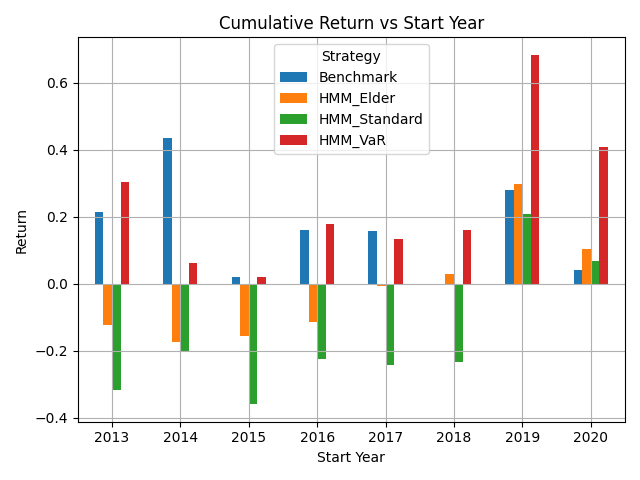
\includegraphics[width=0.8\linewidth]{../main/backtest_result/Return_over_time.png}
    \caption{Cumulative Return Performance across Strategies (until 2025)}
    \label{fig:return_over_time}
\end{figure}

The Figure~\ref{fig:return_over_time} highlight clear differences in return generation, risk exposure, and trading behavior. The HMM + VaR Parity strategy consistently outperforms the rest, particularly from 2015 onwards. Its performance accelerates after 2018, culminating in substantial peak in 2019. This suggests that volatility-aware capital allocation becomes especially effective during periods of heightened market dispersion. In contrast, the standard HMM strategy persistently underperforms, which indicate that regime detection alone, without appropriate risk scaling is insufficient to generate robust returns. 

\begin{figure}[H]
    \centering
    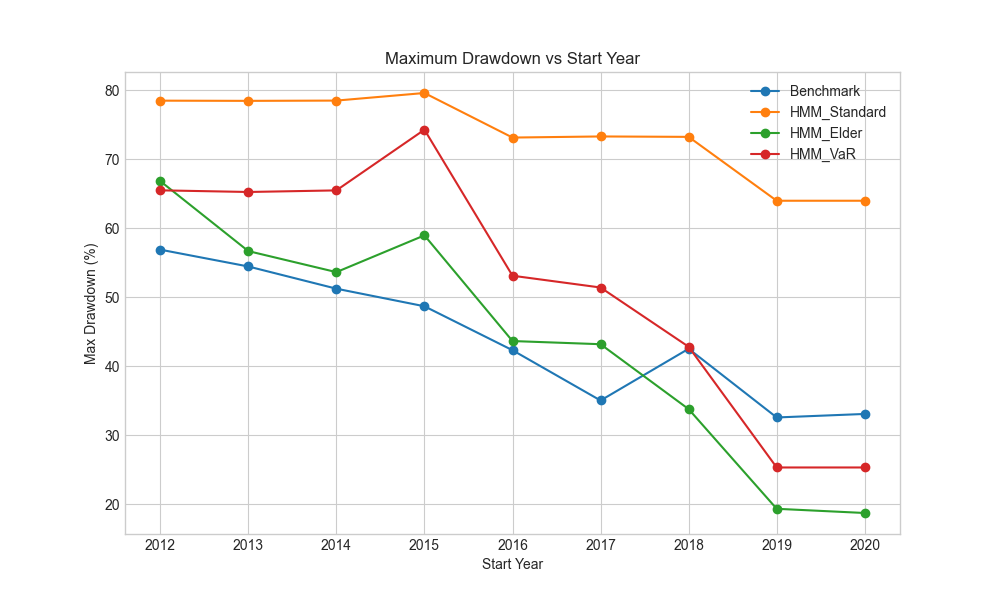
\includegraphics[width=1.0\linewidth]{../main/backtest_result/MaxDD_over_time.png}
    \caption{Max Drawdown vs Starting Year across Strategies}
    \label{fig:max_drawdown_over_time}
\end{figure}

The Figure~\ref{fig:max_drawdown_over_time} highlights the effectiveness of different risk controls. The HMM Standard strategy consistently suffers from severe drawdowns, often exceeding 70\%. The HMM + Elder Rules significantly improves drawdown control, while the HMM + VaR Parity approach achieves the most balanced profile, with drawdowns declines severely after 2018. This shows that volatility scaling and risk budgeting are essential components in mitigating tail risk within regime-switching frameworks.

\begin{figure}[H]
    \centering
    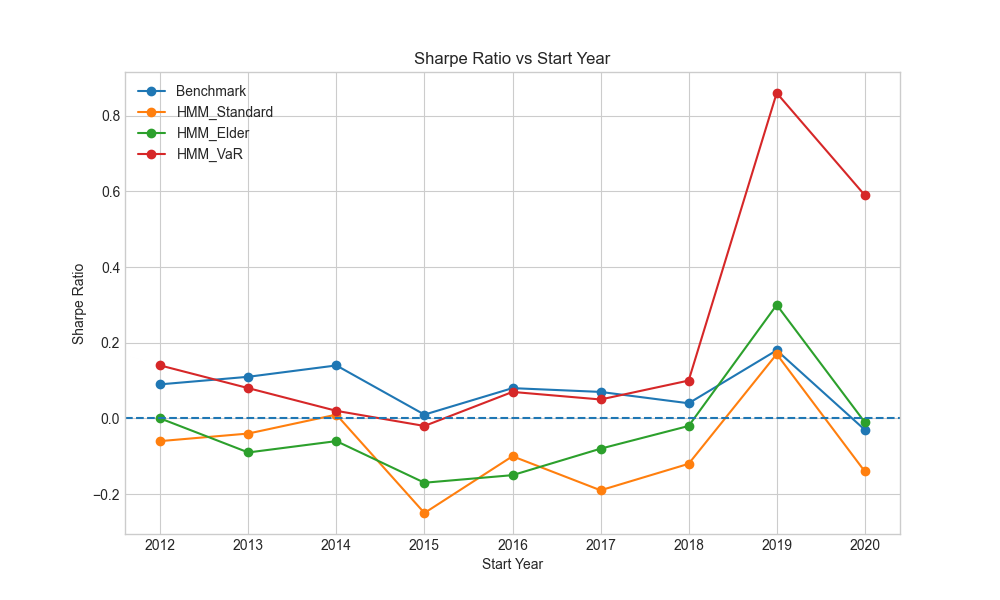
\includegraphics[width=1.0\linewidth]{../main/backtest_result/SharpeRatio_over_time.png}
    \caption{Sharpe Ratio vs Starting Year across Strategies}
    \label{fig:sharpe_ratio_over_time}
\end{figure}

The Figure~\ref{fig:sharpe_ratio_over_time} shows that the HMM Var Parity demonstrates improvement in Sharpe Ratio during later period while most strategies struggle to achieve stable risk-adjusted returns before 2018.  The HMM Elder strategy also shows moderate enhancement, whereas HMM Standard remains consistently weak. Overall, the results indicate that incorporating both regime awareness and volatility-sensitive position sizing is critical for achieving superior risk-adjusted performance, especially when there are multiple shifts in market regimes.

\subsection{Performance Attribution}

To better understand the sources of excess return, we apply the Brinson-Hood-Beebower (BHB) attribution framework, decomposing the active return of the HMM + VaR Parity strategy relative to the market-cap-weighted benchmark into three components: \textit{Allocation}, \textit{Selection}, and \textit{Interaction} effects across GICS sectors.

\begin{figure}[H]
    \centering
    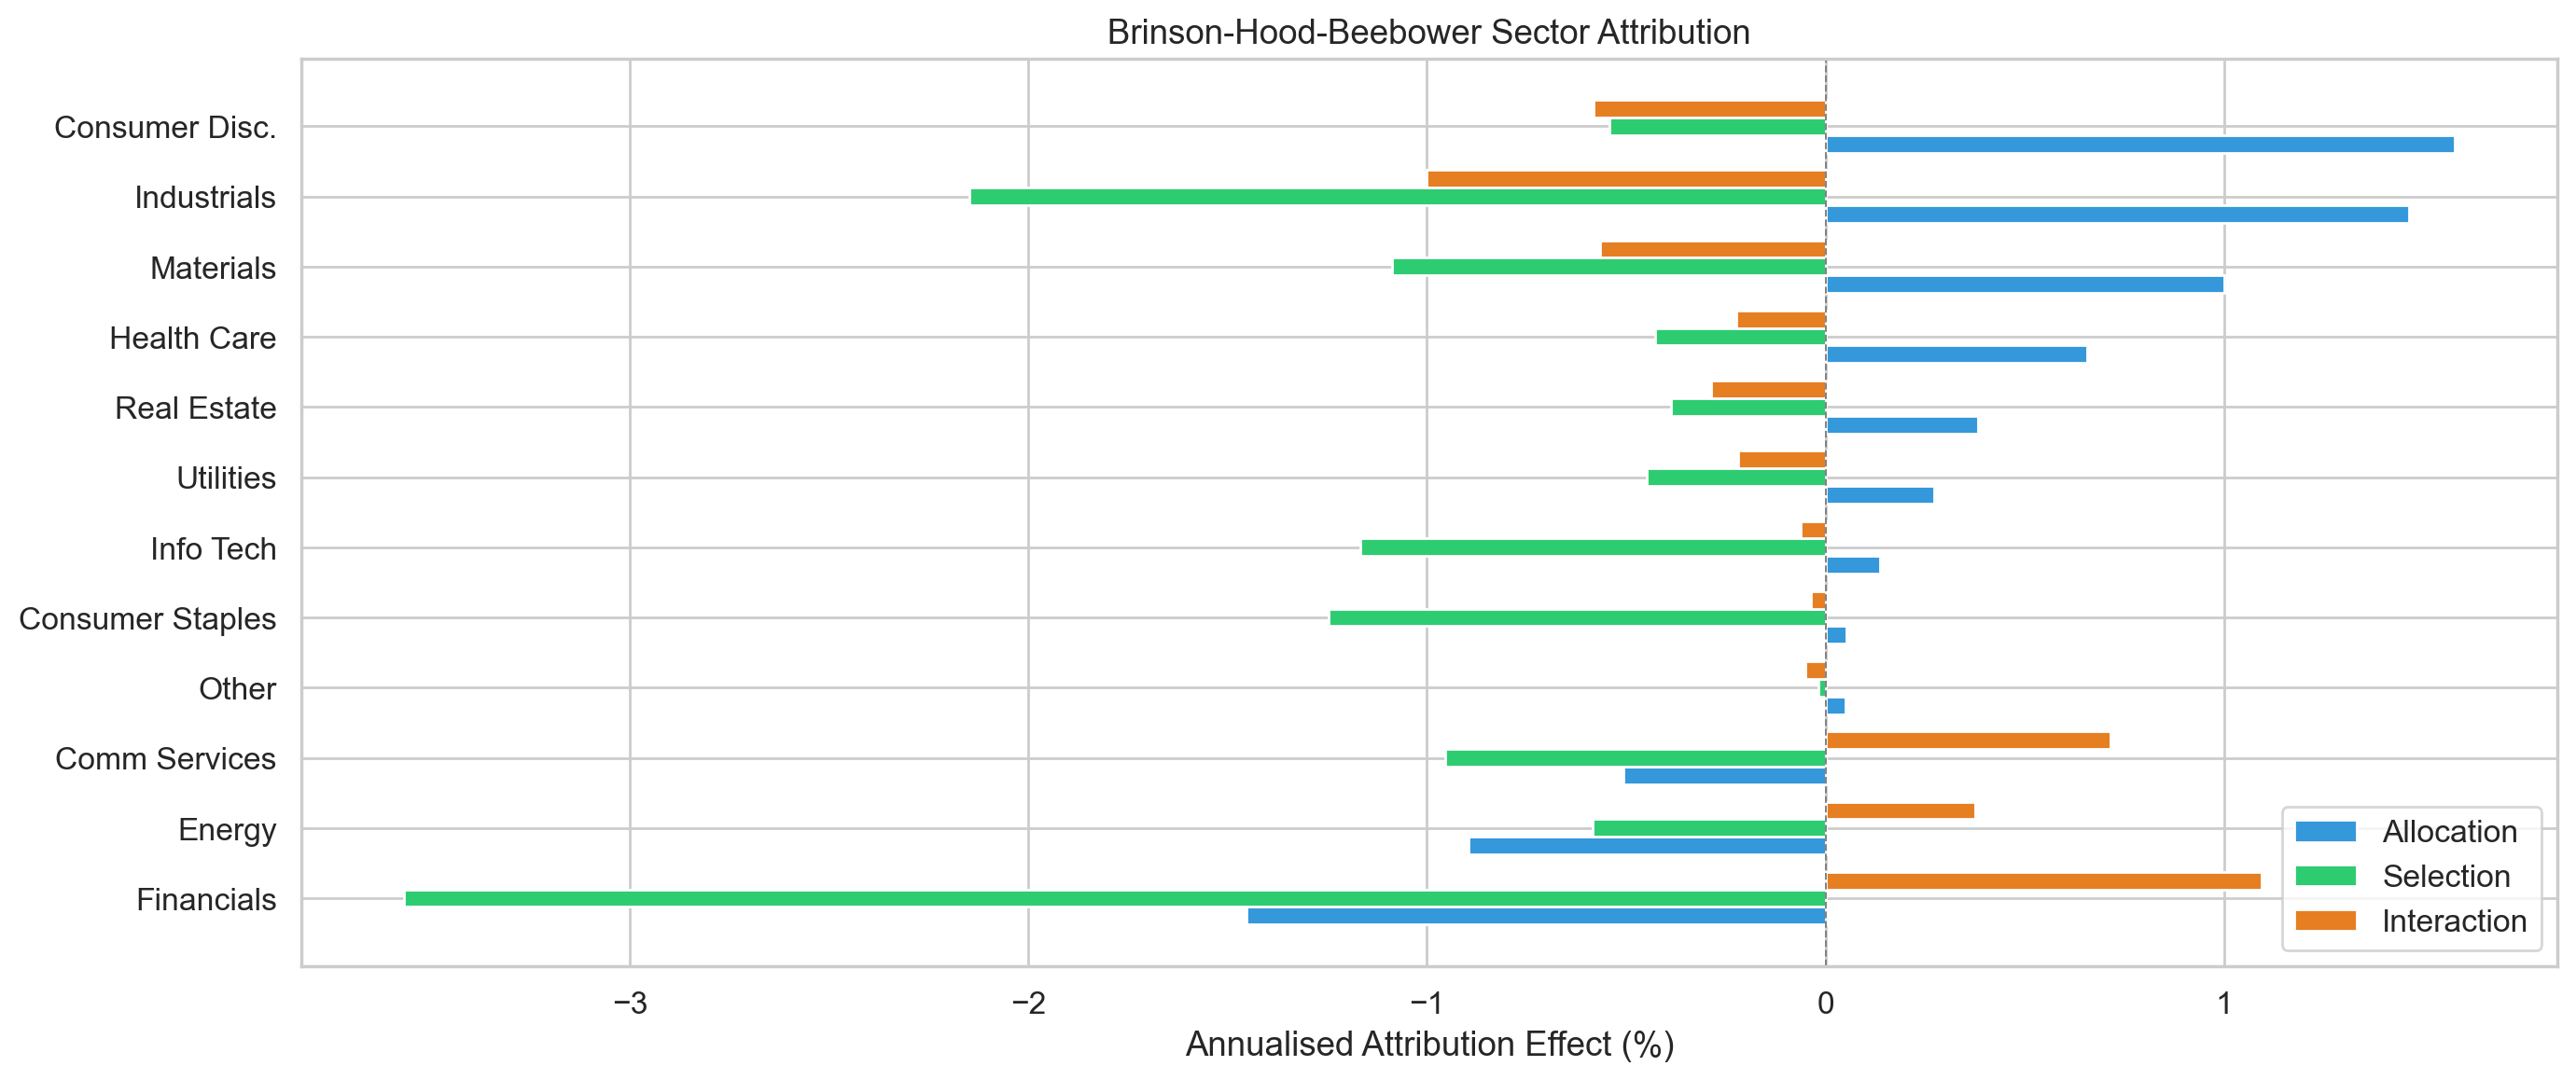
\includegraphics[width=1.0\linewidth]{../main/backtest_result/brinson_sector_attribution.png}
    \caption{Brinson-Hood-Beebower sector attribution of annualised active return.}
    \label{fig:brinson_attribution}
\end{figure}

Figure~\ref{fig:brinson_attribution} reveals several key findings. It was identified that financials caused that largest drag on performance, showing a strongly negative allocation effect of approximately $-3.5\%$ annualised. This indicates that the signal-driven weighting scheme naturally gravitates toward high-capitalisation financial stocks --- which dominate the Chinese A-share universe --- during periods when the sector underperforms. The negative Selection effect within Financials further compounds this, suggesting that the HMM signals do not effectively differentiate between strong and weak names in this sector.

The Consumer Discretionary emerges as the top contributor through a positive Selection effect of roughly $+1.3\%$, implying that the momentum and regime signals successfully identify outperforming stocks within this sector. Industrials exhibits a similar pattern: despite a large negative Allocation effect ($\approx -2.2\%$), the Selection effect ($\approx +1.1\%$) partially offsets the sector-level misallocation.

Health Care shows a meaningful positive Allocation effect ($\approx +0.7\%$), indicating that the strategy correctly overweights this sector during favourable regimes. Conversely, Information Technology and Consumer Staples both display negative Selection effects ($\approx -0.8\%$), suggesting that the HMM signals underperform in picking stocks within these sectors.

Overall, the attribution analysis indicates that the strategy derives more value from intra-sector stock selection than from sector rotation. The Selection bars dominate across most sectors, confirming that the HMM + Hurst signals primarily add alpha through timing individual stock exposures rather than macro-level sector tilts. The concentrated negative allocation in Financials points to a clear avenue for improvement: introducing explicit sector-weight constraints --- such as capping the Financials allocation --- could materially reduce this drag and improve risk-adjusted performance.

\section{Conclusion}
This paper presents a theoretical and empirical framework that bridges the gap between macroeconomic regime modeling and microstructural price behavior. By integrating a Gaussian Hidden Markov Model with the Hurst exponent, the proposed architecture effectively filters out the "noise" that plagues traditional momentum strategies.

Future research could expand this framework from a time-series application (single asset) to a cross-sectional application (multi-asset portfolios). Specifically, calculating the Hurst exponent across an entire equities universe to construct a Smart Momentum Factor—going long only on assets exhibiting both high relative momentum and a Hurst exponent $>$ 0.6— represents a promising frontier for multifactor quantitative modeling.

\printbibliography

\end{document}